\chapter{Generalized Unitarity Bounds}

\begin{flushright}
\small

{\color{chapterpaperrule}\rule{\textwidth}{0.5pt}}

\textit{This chapter is based on Ref.~\cite{Bresciani:2025toe}:}\\[0.5em]
L.~C.~Bresciani, G.~Levati and P.~Paradisi,\\
``Amplitudes and partial wave unitarity bounds,''\\
\href{https://doi.org/10.1103/tp6m-mcyn}{Phys. Rev. D \textbf{113} (2026) no.7, L071702}
%doi:10.1103/tp6m-mcyn
[\href{https://doi.org/10.48550/arXiv.2504.12855}{arXiv:2504.12855} [hep-ph]].

{\color{chapterpaperrule}\rule{\textwidth}{0.5pt}}
\end{flushright}

\section{Formalism\label{sec:PWUB_formalism}}

The partial-wave analysis allows one to project 
a generic amplitude $\ket*{\mathcal A_{i\to f}}$ 
onto a kinematic basis $\ket*{\mathcal B^J_{i\to f}}$
with definite angular momentum $J$ as follows
%
\begin{align}
    \ket*{\mathcal A_{i\to f}} = \sum_J a^J_{i\to f}\, \ket*{\mathcal B^J_{i\to f}}\,,
    \label{eq:pwd}
\end{align}
or, diagrammatically,
\begin{align}
    \begin{tikzpicture}[baseline=(current bounding box.center)]
[place/.style={circle,draw=black,fill=white,thick}]
\node[place] (n1) at (0,0) {$\mathcal A$};
\node[] (n2) at (-1,0) {};
\node[] (n3) at (-1,1) {};
\node[] (n4) at (-1,-1) {};
\draw[->] (n2) -- (n1);
\draw[->] (n3) -- (n1);
\draw[->] (n4) -- (n1);
\node[] (n5) at (1,0) {};
\node[] (n6) at (1,1) {};
\node[] (n7) at (1,-1) {};
\draw[<-] (n5) -- (n1);
\draw[<-] (n6) -- (n1);
\draw[<-] (n7) -- (n1);
\node[] (txti) at (-1,0) {\scriptsize$i$};
\node[] (txtf) at (1,0) {\scriptsize$f$};
\end{tikzpicture}
\; =
\sum_{J}
a^J_{i\to f}\;
\begin{tikzpicture}[baseline=(current bounding box.center)]
[place/.style={circle,draw=black,fill=white,thick}]
\node[place,rectangle] (n1) at (0,0) {$\mathcal B^J$};
\node[] (n2) at (-1,0) {};
\node[] (n3) at (-1,1) {};
\node[] (n4) at (-1,-1) {};
\draw[->] (n2) -- (n1);
\draw[->] (n3) -- (n1);
\draw[->] (n4) -- (n1);
\node[] (n5) at (1,0) {};
\node[] (n6) at (1,1) {};
\node[] (n7) at (1,-1) {};
\draw[<-] (n5) -- (n1);
\draw[<-] (n6) -- (n1);
\draw[<-] (n7) -- (n1);
\node[] (txti) at (-1,0) {\scriptsize$i$};
\node[] (txtf) at (1,0) {\scriptsize$f$};
\end{tikzpicture}\,,
\end{align}
%
where $a^J_{i\to f}$ are the partial-wave coefficients.
%
The fundamental building blocks of such a decomposition are the Poincaré Clebsch-Gordan coefficients $\mathcal C_{\mathcal I \to *}^{J,h}$ defined as~\cite{Jiang:2020rwz}
%
\begin{equation}
    \langle{P,J,h|\mathcal I}\rangle = \mathcal C_{\mathcal I \to *}^{J,h}\,
    \delta^{(4)}\!\left(P-\sum_{i\in\mathcal I}p_i\right)\!\,,
\end{equation}
%
namely the overlap between the multiparticle state $\ket*{\mathcal I}$ and the Poincaré irreducible multiparticle state $\ket*{P,J,h}$, where $h$ denotes the projection of the angular momentum onto the axis of the linear momentum.
The coefficients $\mathcal C_{\mathcal I \to *}^{J,h}$ can be seen as elements of the complex vector space $V_{\mathcal I \to *}$, i.e., $\ket*{\mathcal C_{\mathcal I \to *}^{J,h}}\in V_{\mathcal I \to *}$, and, correspondingly, the angular momentum basis elements are given by
\begin{gather}
    \ket*{\mathcal B^{J}_{i\to f}} = \sum_h \ket*{\mathcal C_{i \to *}^{J,h}} \otimes \ket*{\mathcal C_{* \to f}^{J,h}} \in V_{i\to f}\,,
    \\
    \begin{tikzpicture}[baseline=(current bounding box.center)]
[place/.style={circle,draw=black,fill=white,thick}]
\node[place,rectangle] (n1) at (0,0) {$\mathcal B^J$};
\node[] (n2) at (-1,0) {};
\node[] (n3) at (-1,1) {};
\node[] (n4) at (-1,-1) {};
\draw[->] (n2) -- (n1);
\draw[->] (n3) -- (n1);
\draw[->] (n4) -- (n1);
\node[] (n5) at (1,0) {};
\node[] (n6) at (1,1) {};
\node[] (n7) at (1,-1) {};
\draw[<-] (n5) -- (n1);
\draw[<-] (n6) -- (n1);
\draw[<-] (n7) -- (n1);
\node[] (txti) at (-1,0) {\scriptsize$i$};
\node[] (txtf) at (1,0) {\scriptsize$f$};
\end{tikzpicture}
\; = 
\sum_h 
\;
\begin{tikzpicture}[baseline=(current bounding box.center)]
[place/.style={circle,draw=black,fill=white,thick}]
\node[place,isosceles triangle] (n1) at (0,0) {$\mathcal C^{J,h}$};
\node[] (n2) at (-1,0) {};
\node[] (n3) at (-1,1) {};
\node[] (n4) at (-1,-1) {};
\draw[->] (n2) -- (n1);
\draw[->] (n3) -- (n1);
\draw[->] (n4) -- (n1);
\node[] (txti) at (-1,0) {\scriptsize$i$};
\node[] (txtf) at (3.5,0) {\scriptsize$f$};
\node[place,isosceles triangle,shape border rotate=180] (n5) at (2.5,0) {$\mathcal C^{J,h}$};
\draw[->,double] (n1) to node[above] {\scriptsize$P,J,h$} (n5);
\node[] (n7) at (3.5,0) {};
\node[] (n8) at (3.5,1) {};
\node[] (n9) at (3.5,-1) {};
\draw[<-] (n7) -- (n5);
\draw[<-] (n8) -- (n5);
\draw[<-] (n9) -- (n5);
\end{tikzpicture}\; \in V_{i\to f}\,,
\end{gather}
where
$\ket*{\mathcal C^{J,h}_{* \to \mathcal I}}=\ket*{(\mathcal C^{J,h}_{\mathcal I \to *})^*} \in V_{* \to \mathcal I}$ and $V_{i\to f} = V_{i \to *}\otimes V_{* \to f}$:
\begin{align}
    \langle{P,J,h|i}\rangle &= \mathcal C_{i \to *}^{J,h}\,
    \delta^{(4)}\!\left(P-\sum_{k\in i}p_k\right)=\;
    \begin{tikzpicture}[baseline=(current bounding box.center)]
[place/.style={circle,draw=black,fill=white,thick}]
\node[place,isosceles triangle] (n1) at (0,0) {$\mathcal C^{J,h}$};
\node[] (n2) at (-1,0) {};
\node[] (n3) at (-1,1) {};
\node[] (n4) at (-1,-1) {};
\draw[->] (n2) -- (n1);
\draw[->] (n3) -- (n1);
\draw[->] (n4) -- (n1);
\node[] (txti) at (-1,0) {\scriptsize$i$};
%\node[] (txtf) at (3.5,0) {$f$};
%\node[place,isosceles triangle,shape border rotate=180] (n5) at (2.5,0) {$\mathcal C^{J,\sigma}$};
\node[] (n5) at (1.5,0) {};
\draw[->,double] (n1) to node[above] {\scriptsize$P,J,h$} (n5);
\end{tikzpicture}\;
\in V_{i \to *}\,,
\\
\langle{f|P,J,h}\rangle &= \mathcal C_{* \to f}^{J,h}\,
    \delta^{(4)}\!\left(P-\sum_{k\in f}p_k\right)
    = \;
    \begin{tikzpicture}[baseline=(current bounding box.center)]
    \node[] (n1) at (1,0) {};
        \node[place,isosceles triangle,shape border rotate=180] (n5) at (2.5,0) {$\mathcal C^{J,h}$};
\draw[double,->] (n1) to node[above] {\scriptsize$P,J,h$} (n5);
\node[] (n7) at (3.5,0) {};
\node[] (n8) at (3.5,1) {};
\node[] (n9) at (3.5,-1) {};
\draw[<-] (n7) -- (n5);
\draw[<-] (n8) -- (n5);
\draw[<-] (n9) -- (n5);
\node[] (txtf) at (3.5,0) {\scriptsize$f$};
    \end{tikzpicture}\;\in V_{* \to f}\,.
\end{align}
The partial-wave coefficients $a_{i\to f}^J$ can then be conveniently obtained by extending the inner product 
in $V_{\mathcal I \to *}$~\cite{Shu:2021qlr} to the
vector space $V_{i\to f}$ as follows
%
\begin{align}
    a_{i\to f}^J &= \frac{1}{2J+1}\langle \mathcal B^J_{i\to f}|\mathcal A_{i\to f}\rangle 
    %\nonumber \\
    =
    \frac{1}{2J+1}\int \text{d}\Phi_i\, \text{d}\Phi_f\, \mathcal A_{i\to f}\left(\mathcal B^J_{i\to f}\right)^*
    \nonumber \\
    &= \frac{1}{2J+1}\;
            \scalebox{1}{\begin{tikzpicture}[baseline=(current bounding box.center)]
[place/.style={circle,draw=black,fill=white,thick}]
\node[place] (n1) at (0,0) {$\mathcal A$};
\node[place,rectangle] (n2) at (2,0) {$\mathcal B^J$};
\draw[->] (n1) to [bend left=60] (n2);
\draw[->] (n1) to [bend left=80] (n2);
\draw[->] (n1) to [bend left=100] (n2);
\draw[<-] (n1) to [bend right=60] (n2);
\draw[<-] (n1) to [bend right=80] (n2);
\draw[<-] (n1) to [bend right=100] (n2);
\node[] (t1) at (1,1.35) {};
\node[] (t2) at (1,0.35) {\scriptsize$f$};
\draw[color=gray,very thick,densely dotted] (t1) to [] (t2);
\node[] (t3) at (1,-1.35) {};
\node[] (t4) at (1,-0.35) {\scriptsize$i$};
\draw[color=gray,very thick, densely dotted] (t3) -- (t4);
\end{tikzpicture}}\,,
    \label{eq:partial_wave}
\end{align}
%
where
\begin{equation}
    \dd \Phi_{\mathcal I} = \frac{1}{S_{\mathcal I}} \prod_{k \in \mathcal{I}} \frac{\dd^3 p_k}{(2\pi)^3\, 2E_k}
\end{equation}
refers to the Lorentz-invariant phase-space measure associated with $\ket*{\mathcal I}$ and $S_{\mathcal I}$ is the symmetry factor accounting for identical particles in $\ket{\mathcal{I}}$.\footnote{Explicit parameterizations for the $n$-body phase space in terms of spinor-helicity variables are available in \cite{Zwiebel:2011bx,Mastrolia:2009dr,Cox:2018wce,Larkoski:2020thc,EliasMiro:2020tdv}.}
Notice that we crucially chose the basis normalization
\begin{equation}
    \langle \mathcal B^J_{i\to f}|\mathcal B^{J'}_{i\to f}\rangle = (2J+1)\,\delta^{JJ'}
\end{equation}
in order to obtain the partial-wave unitarity bounds in the standard form.
Indeed, this choice implies
\begin{gather}
    \int \text d \Phi_X\,\ket*{\mathcal B^{J}_{i\to X}}\otimes \ket*{\mathcal B_{X\to f}^{J'}} = \ket*{\mathcal B_{i\to f}^J} \delta^{JJ'}\,,
    \\
    \begin{tikzpicture}[baseline=(current bounding box.center)]
    [place/.style={circle,draw=black,fill=white,thick}]
    \node[place,rectangle] (n1) at (0,0) {$\mathcal B^J$};
    \node[] (n2) at (-1,0) {};
    \node[] (n3) at (-1,1) {};
    \node[] (n4) at (-1,-1) {};
    \draw[->] (n2) -- (n1);
    \draw[->] (n3) -- (n1);
    \draw[->] (n4) -- (n1);
    \node[] (txti) at (-1,0) {\scriptsize$i$};
    \node[place,rectangle] (n5) at (2,0) {$\mathcal B^{J'}$};
    \draw[->] (n1) to[bend left=25] (n5);
    \draw[->] (n1) -- (n5);
    \draw[->] (n1) to[bend right=25] (n5);
    \node[] (cut1) at (1,0.65) {};
    \node[] (cut2) at (1,-0.65) {};
    \draw[color=gray,very thick,densely dotted] (cut1) -- (cut2);
    \node[] (txtX) at (1,0.70) {\scriptsize$X$};
    \node[] (n6) at (3,0) {};
    \node[] (n7) at (3,1) {};
    \node[] (n8) at (3,-1) {};
    \draw[<-] (n6) -- (n5);
    \draw[<-] (n7) -- (n5);
    \draw[<-] (n8) -- (n5);
    \node[] (txtf) at (3,0) {\scriptsize$f$};
    \end{tikzpicture}
    \; = \;
    \begin{tikzpicture}[baseline=(current bounding box.center)]
    [place/.style={circle,draw=black,fill=white,thick}]
    \node[place,rectangle] (n1) at (0,0) {$\mathcal B^J$};
    \node[] (n2) at (-1,0) {};
    \node[] (n3) at (-1,1) {};
    \node[] (n4) at (-1,-1) {};
    \draw[->] (n2) -- (n1);
    \draw[->] (n3) -- (n1);
    \draw[->] (n4) -- (n1);
    \node[] (n5) at (1,0) {};
    \node[] (n6) at (1,1) {};
    \node[] (n7) at (1,-1) {};
    \draw[<-] (n5) -- (n1);
    \draw[<-] (n6) -- (n1);
    \draw[<-] (n7) -- (n1);
    \node[] (txti) at (-1,0) {\scriptsize$i$};
    \node[] (txtf) at (1,0) {\scriptsize$f$};
    \end{tikzpicture}
    \; \delta^{JJ'}\,,
\end{gather}
%
which, when applied to the generalized optical theorem,
%
\begin{gather}
    \ket*{\mathcal A_{i\to f}} - \ket*{\mathcal A_{f\to i}^*} = i \sum_X \int \text d \Phi_X\, \ket*{\mathcal A_{i\to X}}\otimes\ket*{\mathcal A_{f\to X}^* }\,,
    \\
    \begin{tikzpicture}[baseline=(current bounding box.center)]
    [place/.style={circle,draw=black,fill=white,thick}]
    \node[place] (n1) at (0,0) {$\mathcal A$};
    \node[] (n2) at (-1,0) {};
    \node[] (n3) at (-1,1) {};
    \node[] (n4) at (-1,-1) {};
    \draw[->] (n2) -- (n1);
    \draw[->] (n3) -- (n1);
    \draw[->] (n4) -- (n1);
    \node[] (n5) at (1,0) {};
    \node[] (n6) at (1,1) {};
    \node[] (n7) at (1,-1) {};
    \draw[<-] (n5) -- (n1);
    \draw[<-] (n6) -- (n1);
    \draw[<-] (n7) -- (n1);
    \node[] (txti) at (-1,0) {\scriptsize$i$};
    \node[] (txtf) at (1,0) {\scriptsize$f$};
    \end{tikzpicture}
    \;-\;
    \begin{tikzpicture}[baseline=(current bounding box.center)]
    [place/.style={circle,draw=black,fill=white,thick}]
    \node[place] (n1) at (0,0) {$\mathcal A{}^\dagger$};
    \node[] (n2) at (-1,0) {};
    \node[] (n3) at (-1,1) {};
    \node[] (n4) at (-1,-1) {};
    \draw[->] (n2) -- (n1);
    \draw[->] (n3) -- (n1);
    \draw[->] (n4) -- (n1);
    \node[] (n5) at (1,0) {};
    \node[] (n6) at (1,1) {};
    \node[] (n7) at (1,-1) {};
    \draw[<-] (n5) -- (n1);
    \draw[<-] (n6) -- (n1);
    \draw[<-] (n7) -- (n1);
    \node[] (txtf) at (-1,0) {\scriptsize$i$};
    \node[] (txti) at (1,0) {\scriptsize$f$};
    \end{tikzpicture}\;
     = 
    i\sum_X \;
    \begin{tikzpicture}[baseline=(current bounding box.center)]
    [place/.style={circle,draw=black,fill=white,thick}]
    \node[place] (n1) at (0,0) {$\mathcal A$};
    \node[] (n2) at (-1,0) {};
    \node[] (n3) at (-1,1) {};
    \node[] (n4) at (-1,-1) {};
    \draw[->] (n2) -- (n1);
    \draw[->] (n3) -- (n1);
    \draw[->] (n4) -- (n1);
    \node[] (txti) at (-1,0) {\scriptsize$i$};
    \node[place] (n5) at (2,0) {$\mathcal A{}^\dagger$};
    \draw[->] (n1) to[bend left=25] (n5);
    \draw[->] (n1) -- (n5);
    \draw[->] (n1) to[bend right=25] (n5);
    \node[] (cut1) at (1,0.65) {};
    \node[] (cut2) at (1,-0.65) {};
    \draw[color=gray,very thick,densely dotted] (cut1) -- (cut2);
    \node[] (txtX) at (1,0.70) {\scriptsize$X$};
    \node[] (n6) at (3,0) {};
    \node[] (n7) at (3,1) {};
    \node[] (n8) at (3,-1) {};
    \draw[<-] (n6) -- (n5);
    \draw[<-] (n7) -- (n5);
    \draw[<-] (n8) -- (n5);
    \node[] (txtf) at (3,0) {\scriptsize$f$};
    \end{tikzpicture}
\end{gather}
leads to  
%
\begin{equation}
    a_{i\to f}^J - \left(a_{f\to i}^J\right)^* = i \sum_X a_{i\to X}^{J} \left(a_{f\to X}^{J}\right)^*
\end{equation}
%
and, in turn, to the partial-wave unitarity bounds
%
\begin{gather}
    \abs*{\Re a_{i\to i}^J}  \le 1 \,,\qquad  0 \le \Im a_{i\to i}^J \le 2\,,\qquad
%    \\
    \abs*{a^J_{i\to f} }\le 1 \,,
\end{gather}
%
where $i\neq f$.
%
In practice, the determination of the angular momentum basis elements $\ket*{\mathcal B^{J}_{i\to f}}$, required by the partial-wave decomposition,
can be achieved without passing through the Poincaré Clebsch-Gordan coefficients $\ket*{\mathcal C_{\mathcal I \to *}^{J,h}}$, as one can proceed as follows:
%
\begin{enumerate}
    \item Find a set of kinematic monomials in spinor-helicity variables that are consistent with the particle helicities, span the vector space $V_{i\to f}$, and are independent after accounting for momentum conservation and Schouten identities.\footnote{Public Mathematica packages that allow one to perform this task are available in~\cite{DeAngelis:2022qco,Li:2022tec}.}
    \item Apply the Pauli-Lubanski operator squared~\cite{Witten:2003nn}
    %
    \begin{align}
    \mathbb W^2_{\mathcal I} &= \frac{1}{8}\mathbb P_{\mathcal I}^2 \left(\epsilon^{\alpha\gamma}\epsilon^{\beta\delta}\mathbb M_{\mathcal I,\alpha\beta}\mathbb M_{\mathcal I,\gamma\delta}+\epsilon^{\dot\alpha\dot\gamma}\epsilon^{\dot\beta\dot\delta}\widetilde{\mathbb M}_{\mathcal I,\dot\alpha\dot\beta}\widetilde{\mathbb M}_{\mathcal I,\dot\gamma\dot\delta}\right)
    %\nonumber \\&\quad 
    +\frac{1}{4}\mathbb P_{\mathcal I}^{\alpha\dot\alpha}\mathbb P_{\mathcal I}^{\beta\dot\beta}\mathbb M_{\mathcal I,\alpha\beta}\widetilde{\mathbb M}_{\mathcal I,\dot\alpha\dot\beta}\,,
    \label{eq:PLoperator}
\end{align}
where
\begin{align}
    \mathbb P_{\mathcal I}^{\alpha\dot\alpha} &= \sum_{i\in \mathcal I}\lambda_i^\alpha \widetilde \lambda_i^{\dot\alpha}\,,\\
    \mathbb M_{\mathcal I}^{\alpha\beta} &= \sum_{i\in \mathcal I}\left(\lambda_{i}^\alpha\frac{\partial}{\partial \lambda_{i,\beta}}+\lambda_{i}^\beta \frac{\partial}{\partial \lambda_{i,\alpha}}\right)\,,\\
    \widetilde{\mathbb M}_{\mathcal I}^{\dot\alpha\dot\beta} &= \sum_{i\in \mathcal I}\left(\widetilde\lambda_{i}^{\dot\alpha}\frac{\partial}{\partial \widetilde\lambda_{i,\dot\beta}}+\widetilde\lambda_{i}^{\dot\beta}\frac{\partial}{\partial \widetilde\lambda_{i,\dot\alpha}}\right)\,,
\end{align}
and $\mathcal I=i,f$,\footnote{We use the convention $\epsilon^{12}=\epsilon^{\dot 1 \dot 2} =  1$, where spinor indices are raised and lowered as $\lambda ^\alpha = \epsilon^{\alpha\beta}\lambda_\beta$ and $\widetilde\lambda_{\dot \alpha} = \epsilon_{\dot\alpha \dot\beta}\widetilde\lambda^{\dot\beta}$. Angle and square brackets are then defined as $\agl{i}{j} = \lambda_i^\alpha \lambda_{j,\alpha}$ and $\sqr{i}{j} = \widetilde\lambda_{i,\dot\alpha}\widetilde\lambda_j^{\dot\alpha}$, respectively.} to these monomials and construct the associated matrix.
%
\item Find the eigenvectors of the above matrix and the associated values of angular momentum from the Casimir eigenvalues $-P^2_{\mathcal I}J_{\mathcal I}(J_{\mathcal I}+1)$.
\item Normalize the elements of the resulting orthogonal basis so that their norm is equal to $\sqrt{2J_{\mathcal I}+1}$.
\end{enumerate}

As expected, for $2\to 2$ scattering processes, the basis elements $\ket*{\mathcal B^{J}_{i\to f}}$ are proportional to the Wigner $d$-matrices~\cite{Jiang:2020rwz}. 
Moreover, we have explicitly verified that the
partial-wave coefficients for $N\to M$ scattering processes (with $N,M \geq 2$) exactly reproduce the elements of the reduced scattering matrix~\cite{Chang:2019vez,Falkowski:2019tft,Cohen:2021ucp,Mahmud:2025wye}, which captures only the $s$-wave contribution.

As an interesting result of our analysis, in Appendix~\ref{app:2-to-3_basis} we report the angular momentum basis for $2 \to 3$ amplitudes that holds for generic values of $J$.

\section{Effective Field Theory of Gravity and Light-by-Light Scattering}

As a first application of the above method, we analyze the unitarity bounds for the EFT of gravity and light-by-light scattering involving operators with four gravitons and photons, respectively.
%
The versatility of the spinor-helicity formalism in handling particles of arbitrary spin~\cite{Arkani-Hamed:2017jhn} allows us to approach the problem in a unified manner.

We focus on the P- and CP-violating Lagrangian:
\begin{equation}
\label{eq:Lag-quartic}
    \frac{\mathcal L^{(S)}}{\sqrt{-g}} = c_1^{(S)}\,( \mathcal Q^{(S)})^2 + c_2^{(S)}\, (\widetilde{\mathcal Q}^{(S)})^2 + c_3^{(S)}\,  \mathcal Q^{(S)} \,\widetilde{\mathcal Q}^{(S)}
\end{equation}
%
where
%
\begin{align}
    \mathcal Q^{(1)} &= F_{\mu\nu}\,F^{\mu\nu},
    &
    \widetilde{\mathcal Q}^{(1)} &= F_{\mu\nu}\,\widetilde F^{\mu\nu},\\
    \mathcal Q^{(2)} &= \Mpl^2\, R_{\mu\nu\rho\sigma}\,R^{\mu\nu\rho\sigma},
    &
    \widetilde{\mathcal Q}^{(2)} &= \Mpl^2\, R_{\mu\nu\rho\sigma}\,\widetilde R^{\mu\nu\rho\sigma},
\end{align}
%
$\widetilde F_{\mu\nu}=\frac{1}{2} \epsilon_{\mu\nu\rho\sigma}F^{\rho\sigma}$ is the dual photon field-strength tensor, $\widetilde R_{\mu\nu\rho\sigma} = \frac{1}{2} \epsilon_{\mu\nu\alpha\beta}R^{\alpha\beta}{}_{\rho\sigma}$ is the dual Riemann tensor,\footnote{The convention for the Levi-Civita tensor is $\epsilon^{0123}=1/\sqrt{-g}$.} $\Mpl^2=(8\pi G_{\text{N}})^{-1}$ is the Planck mass squared,
and $c_i^{(S)}$ are dimensionful Wilson coefficients with $[c_i^{(S)}]=-4S$. 
%
For $S=1$, we recover the electromagnetic Euler-Heisenberg Lagrangian~\cite{Heisenberg:1936nmg}, while, for $S=2$, we obtain the eight-derivative corrections to the gravitational Einstein-Hilbert action~\cite{Endlich:2017tqa}.
In both cases, the three operators appearing in Eq.~\eqref{eq:Lag-quartic} constitute 
a basis for such effective dimension-$(4S+4)$ operators~\cite{Ruhdorfer:2019qmk,Li:2023wdz}.

Denoting by $i=\{(1^{+S},2^{+S})$, $ (1^{+S},2^{-S})$, $ (1^{-S},2^{-S})\}$ all the possible initial two-particle states and by $f=\{(3^{+S},4^{+S})$, $ (3^{+S},4^{-S})$, $(3^{-S},4^{-S})\}$ the final ones, the full four-particle scattering matrix reads
%
\begin{equation}\label{eq:amplitude}
    \ket*{\mathcal A_{i\to f}} = 
    \begin{pmatrix}
        \substack{8c_+^{(S)}\agl{1}{2}^{2S}\sqr{3}{4}^{2S}} & 0 
        & \substack{8c_-^{(S)}(\agl{1}{2}^{2S}\agl{3}{4}^{2S}\\+\agl{1}{3}^{2S}\agl{2}{4}^{2S}+\agl{1}{4}^{2S}\agl{2}{3}^{2S})}
        \\
        0 & \substack{8c_+^{(S)}\agl{1}{4}^{2S}\sqr{2}{3}^{2S}} 
        & 0
        \\
        \substack{8(c_-^{(S)})^*(\sqr{1}{2}^{2S}\sqr{3}{4}^{2S}\\+\sqr{1}{3}^{2S}\sqr{2}{4}^{2S}+\sqr{1}{4}^{2S}\sqr{2}{3}^{2S})} & 0 
        & \substack{8c_+^{(S)}\agl{3}{4}^{2S}\sqr{1}{2}^{2S}}
    \end{pmatrix}
\end{equation}
%
with 
\begin{equation}
    c_+^{(S)}= c_1^{(S)} + c_2^{(S)}\in \mathbb{R} \,, \qquad
    c_-^{(S)}= c_1^{(S)} - c_2^{(S)} + i c_3^{(S)}\in \mathbb{C}\,.
\end{equation}
%
A simple way to obtain it relies on writing the photon field strength in spinor space as 
\begin{equation}
    F_{\alpha \dot \alpha \beta \dot \beta} \sim \epsilon_{\alpha\beta}\widetilde\lambda_{\dot \alpha}\widetilde\lambda_{\dot \beta}+\epsilon_{\dot\alpha\dot\beta}\lambda_\alpha \lambda_\beta
\end{equation}
and similarly for the Riemann tensor \cite{Arkani-Hamed:2020blm}
\begin{equation}
    R_{\alpha\dot\alpha\beta\dot\beta\gamma\dot\gamma\delta\dot\delta}\sim \epsilon_{\alpha\beta}\epsilon_{\gamma\delta}\widetilde\lambda_{\dot\alpha}\widetilde\lambda_{\dot\beta}\widetilde\lambda_{\dot\gamma}\widetilde\lambda_{\dot\delta} + \epsilon_{\dot\alpha\dot\beta}\epsilon_{\dot\gamma\dot\delta}\lambda_{\alpha}\lambda_{\beta}\lambda_{\gamma}\lambda_{\delta}\,.
\end{equation}

The kinematic vector space for the maximally helicity-violating amplitude in Eq.~\eqref{eq:amplitude}, i.e., $\mathcal A_{1^{-S},2^{-S}\to 3^{+S},4^{+S}}$, has dimension $2S+1$ and is spanned by $\{\ket*{m_k}\}_{k=1}^{2S+1}$, with
%
\begin{equation}
    \ket*{m_k} = \sqr{1}{2}^{2S-k+1}\sqr{1}{4}^{k-1}\sqr{2}{3}^{k-1}\sqr{3}{4}^{2S-k+1} \,,
\end{equation}
%
which constitutes a basis.
Of course, the same is true for $\mathcal A_{1^{+S},2^{+S}\to 3^{-S},4^{-S}}$, provided that all the square inner products are substituted with angle ones.
%
In this basis, the Pauli-Lubanski operator squared of Eq.~\eqref{eq:PLoperator} is represented by an upper bidiagonal matrix:
%
\begin{equation}
    \mathbb W^2_{12}=-s 
    \begin{pmatrix}
        0 & 1 & 0 & \cdots & \cdots & \cdots & 0 \\
        0 & 2 & 4 & \ddots & \ddots & \ddots & \vdots \\
        0 & 0 & 6 & 9 & \ddots & \ddots & \vdots \\
        \vdots & \ddots & 0 & 12 & 16 &\ddots & \vdots \\
        \vdots & \ddots & \ddots & 0 & 20 & \ddots & 0 \\
        \vdots & \ddots & \ddots & \ddots & \ddots & \ddots & 4S^2 \\
        0 & \cdots & \cdots & \cdots & 0 & 0 & 2S(2S+1) 
    \end{pmatrix}
\end{equation}
%
where $s=(p_1+p_2)^2$.
Indeed, it acts on the basis monomials $\ket*{m_k}$, with $k>1$, as
%
\begin{multline}
    \mathbb W^2_{12} \ket*{m_k} = -s
    \frac{k-1}{2}\sqr{1}{2}^{2S-k+1}\sqr{1}{4}^{k-2}\sqr{2}{3}^{k-2}\sqr{3}{4}^{2S-k+1} \\
     \times 
    \big((k+1)\sqr{1}{4}\sqr{2}{3}+(k-1)(\sqr{1}{3}\sqr{2}{4}+\sqr{1}{2}\sqr{3}{4})\big)\,,
\end{multline}
%
which, once we use the Schouten identity $\sqr{1}{3}\sqr{2}{4}=\sqr{1}{2}\sqr{3}{4}+\sqr{1}{4}\sqr{2}{3}$, becomes
%
\begin{equation}
   \mathbb W^2_{12} \ket*{m_k} = -s\left((k-1)^2\ket*{m_{k-1}}+k(k-1)\ket*{m_k}\right)\,.
\end{equation}
%
The eigenvalues of this matrix are given by its diagonal entries and correspond to $J_{12}=0,1,\dotsc,2S$. 

Instead, for all the amplitudes in Eq.~\eqref{eq:amplitude} that are proportional to $c_+^{(S)}$, the dimension of the kinematic vector space is $1$, and thus such amplitudes have a definite angular momentum.
%
In particular, $\mathcal A_{1^{\pm S},2^{\pm S}\to 3^{\pm S},4^{\pm S}}$ has $J_{12}=0$, while $\mathcal A_{1^{+ S},2^{- S}\to 3^{+ S},4^{- S}}$ has $J_{12}=2S$, since 
%
\begin{equation}
    \mathbb  W^2_{12}\agl{1}{2}^{2S}\sqr{3}{4}^{2S} = \mathbb  W^2_{12}\agl{3}{4}^{2S}\sqr{1}{2}^{2S}=0
\end{equation}
%
and 
%
\begin{align}
    \mathbb  W^2_{12}\agl{1}{4}^{2S}\sqr{2}{3}^{2S} = -s[2S(2S+1)]\agl{1}{4}^{2S}\sqr{2}{3}^{2S}\,.
\end{align}

The normalized eigenvectors corresponding to $J_{12}=0$ are then
%
\begin{equation}
    \ket*{\mathcal B_{i\to f}^0} 
    =
    \frac{16\pi}{s^{2S}}
    \begin{pmatrix}
        \agl{1}{2}^{2S}\sqr{3}{4}^{2S} & 0 
        & \agl{1}{2}^{2S}\agl{3}{4}^{2S}\\
        0 & 0 
        & 0\\
        \sqr{1}{2}^{2S}\sqr{3}{4}^{2S} & 0 
        & \sqr{1}{2}^{2S}\agl{3}{4}^{2S}
        \end{pmatrix}\,,
\end{equation}
%
and, by projecting the amplitudes in Eq.~\eqref{eq:amplitude} onto them, it follows that the corresponding partial waves read\footnote{
In this case, the phase space integral can be achieved, e.g., by parameterizing the final-state spinors as~\cite{Mastrolia:2009dr,Bresciani:2024shu}
%
\begin{equation}
    \begin{pmatrix}
        \lambda_3 \\ \lambda_4
    \end{pmatrix}
    =
    \frac{1}{\sqrt{1+z\bar z}}
    \begin{pmatrix}
        1 & \bar z \\
        -z & 1
    \end{pmatrix}
    \begin{pmatrix}
        \lambda_1 \\ \lambda_2
    \end{pmatrix}
\end{equation}
and writing the phase space measure as 
\begin{equation}
    \int \text{d}\Phi_{34} =-\frac{1}{2} \frac{1}{8\pi}\oint \frac{\text{d}z}{2\pi i}\int \frac{\text{d}\bar z}{(1+z\bar z)^2}\,,
\end{equation}
%
where we included the $1/2$ symmetry factor due to indistinguishable particles.
This yields the factors
\begin{equation}
    -\Res_{z=0}\int \text{d}\bar z\frac{1+(z\bar z)^{2S}+(1+z\bar z)^{2S}}{(1+z\bar z)^{2S+2}} = \frac{2S+3}{2S+1}
\end{equation}
that appear in Eq.~\eqref{eq:partialwavecoeffs}.}
%
\begin{equation}\label{eq:partialwavecoeffs}
    a^{0}_{i\to f} =
    \frac{s^{2S}}{2\pi}
    \begin{pmatrix}
        c_+^{(S)} & 0 
        & \frac{2S+3}{2S+1}c_-^{(S)} \\
        0 & 0 
        & 0\\
        \frac{2S+3}{2S+1}(c_-^{(S)})^* & 0 
        & c_+^{(S)}
    \end{pmatrix}\,,
\end{equation}
%
whose non-vanishing eigenvalues are
%
\begin{equation}
    \frac{s^{2S}}{2\pi}\left(c_+^{(S)}\pm \frac{2S+3}{2S+1}|c_-^{(S)}| \right)\,.
\end{equation}
%
As a result, we find that the strongest unitarity bound is provided by the partial wave with $J_{12}=0$:
%
\begin{equation}
\label{eq:PUbounds}
    \mathscr{U}:\qquad \frac{s^{2S}}{2\pi}\left(|c_+^{(S)}|+\frac{2S+3}{2S+1}|c_-^{(S)}|\right) \le 1\,.
\end{equation}
The regions of the parameter space satisfying the partial-wave unitarity condition of Eq.~\eqref{eq:PUbounds} are shown in red in Figure~\ref{fig:s1} for the cases of $S=1,2$, and in the left panels of Figures \ref{fig:s1_v2} and \ref{fig:s2_v2}.\footnote{In deriving these bounds for the gravitational EFT ($S=2$), we explicitly neglected the universal long-range contribution from single-graviton exchange
\begin{equation}
    \ket*{\mathcal A_{1^{+2},2^{+2} \to 3^{+2},4^{+2}}} = \frac{1}{\Mpl^2}\frac{\agl{1}{2}^4 \sqr{3}{4}^4}{stu}\,,
\end{equation}
responsible for the well-known forward and backward singularities that induce infrared divergences in the partial-wave projections of the scattering amplitude. Such divergences are a well-understood feature of long-range interactions and can be systematically handled by factoring out a universal infrared-divergent phase \cite{Weinberg:1965nx} common to all partial waves. This universal phase, which arises from the resummation of iterated single-graviton exchange (the gravitational Born series), does not affect physical observables and can be stripped from the $S$-matrix, as done for example in \cite{Blas:2020dyg,Bellazzini:2025bay}, yielding infrared-finite amplitudes suitable for unitarity and positivity analyses, and leaving the bounds presented here robust. The resolution scale $\mathcal E$ introduced by this procedure \cite{Bellazzini:2025bay} admits a physical interpretation as the energy resolution of a macroscopic detector for soft gravitons. 
Alternative approaches to deal with the above singularity include the smearing method of Ref.~\cite{Caron-Huot:2021rmr} and the dimensional reduction technique of Ref.~\cite{Bellazzini:2019xts}.}

\begin{figure}[tb]
\centering
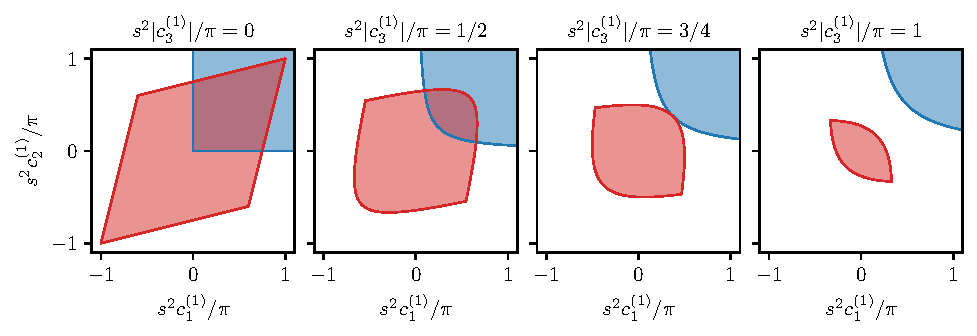
\includegraphics[width=\textwidth]{images/s1_plots_v3.pdf}
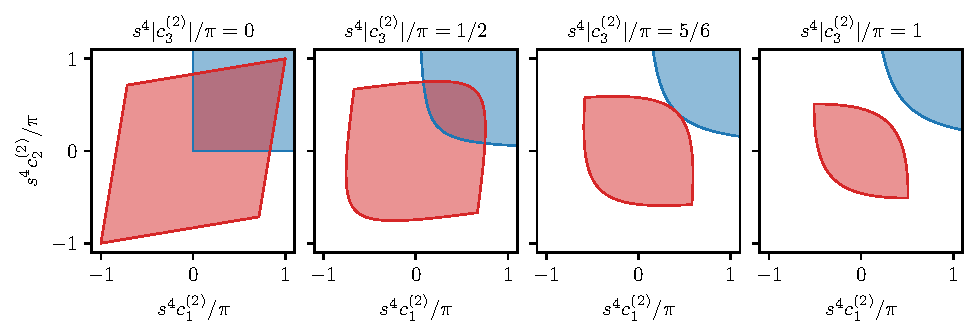
\includegraphics[width=\textwidth]{images/s2_plots_v3.pdf}
\caption{Regions allowed by partial-wave unitarity bounds (red, Eq.~\eqref{eq:PUbounds}) 
and positivity bounds (blue, Eq.~\eqref{eq:positivitybounds}) for the Euler-Heisenberg EFT
(upper panel, $S=1$) and the EFT of gravity (lower panel, $S=2$), in the
$(s^{2S}c_{1}^{(S)},s^{2S}c_{2}^{(S)})$ plane for different values of $s^{2S}c_3^{(S)}$.
\label{fig:s1}}
\end{figure}

\begin{figure}[tb]
    \centering
    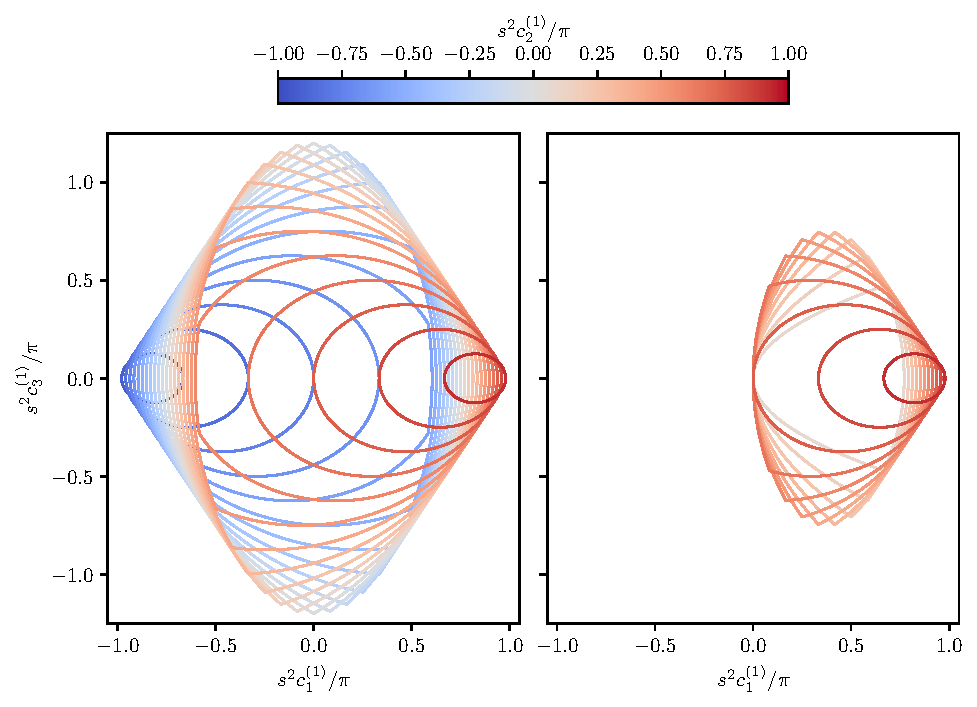
\includegraphics[scale = 0.90]{images/s1_plots_v2.pdf}
    \caption{Contours of the regions allowed by the partial-wave unitarity bounds (left panel, Eq.~\eqref{eq:PUbounds}) combined with the positivity constraints (right panel, Eq.~\eqref{eq:positivitybounds}) for the Euler-Heisenberg EFT ($S=1$) in the $(s^{2}c_{1}^{(1)},s^{2}c_{3}^{(1)})$ plane and computed for different values of $s^{2}c_2^{(1)}$.}
    \label{fig:s1_v2}
\end{figure}

\begin{figure}[tb]
    \centering
    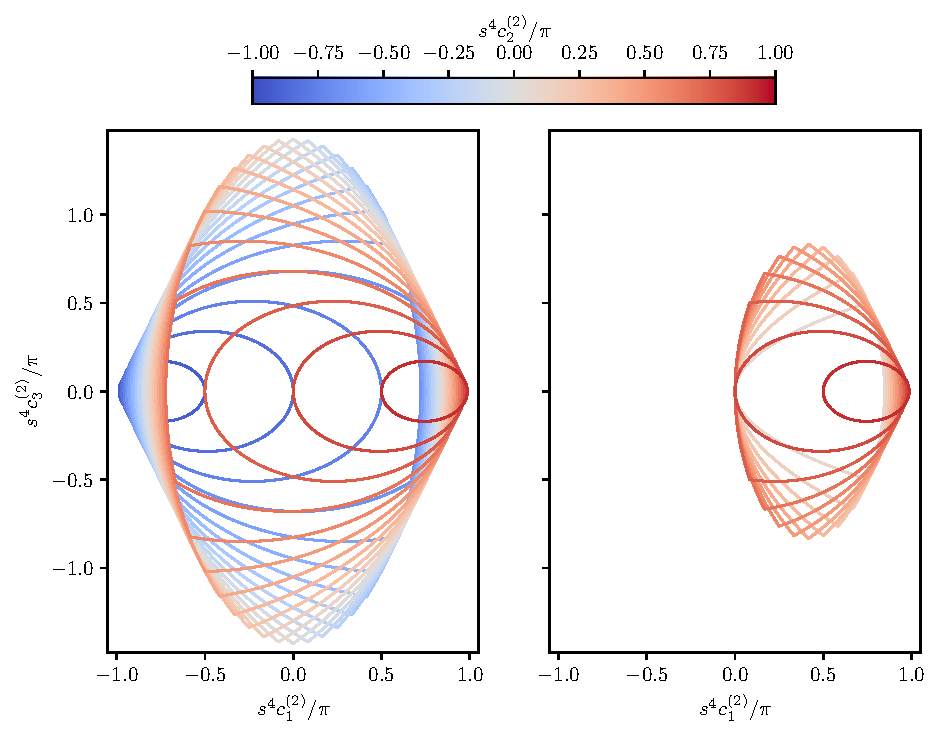
\includegraphics[scale = 0.90]{images/s2_plots_v2.pdf}
    \caption{Contours of the regions allowed by the partial-wave unitarity bounds (left panel, Eq.~\eqref{eq:PUbounds}) combined with the positivity constraints (right panel, Eq.~\eqref{eq:positivitybounds}) for the EFT of gravity ($S=2$) in the $(s^{4}c_{1}^{(2)},s^{4}c_{3}^{(2)})$ plane and computed for different values of $s^{4}c_2^{(2)}$.}
    \label{fig:s2_v2}
\end{figure}

Additional and complementary constraints on the EFT parameter space are represented by positivity bounds, which stem from the analyticity and causality of scattering amplitudes~\cite{Adams:2006sv}. In particular, they impose specific inequalities on the Wilson coefficients to ensure compatibility with a well-behaved UV completion.
%
In our scenarios, they read $\abs*{c_-^{(S)}} \le c_+^{(S)}$, or, equivalently,
%
\begin{align}
\label{eq:positivitybounds}
    \mathscr{P}: \qquad 
    c_{1,2}^{(S)} \ge 0 \,\,\,\,\,\text{and}\,\,\,\,\,
    (c_3^{(S)})^2 \le 4\, c_{1}^{(S)} c_{2}^{(S)}\,,
\end{align}
%
and are valid for both $S=1$~\cite{Adams:2006sv,Rebhan:2017zdx,Remmen:2019cyz,Henriksson:2021ymi,Arkani-Hamed:2020blm} 
and $S=2$~\cite{Gruzinov:2006ie,Bellazzini:2015cra,Endlich:2017tqa,Arkani-Hamed:2020blm,Caron-Huot:2022ugt,Bellazzini:2022wzv}.
%
The regions satisfying these positivity constraints are shown in blue in Figure~\ref{fig:s1} for the cases of $S=1,2$, and in the right panels of Figures \ref{fig:s1_v2} and \ref{fig:s2_v2}.
%The blue regions in Figure~\ref{fig:s1} satisfy positivity bounds. 
Interestingly, we emphasize that the viable parameter space is significantly reduced once both positivity and partial-wave unitarity bounds are imposed. 

To highlight the impact of positivity bounds, we compare the volume of the parameter space allowed by unitarity, $\text{Vol}(\mathscr U)$, with the one obtained after imposing the positivity constraints, $\text{Vol}(\mathscr U \cap \mathscr P)$.
In particular, for fixed values of the center-of-mass energy, we find
%
\begin{equation}
\frac{\text{Vol}(\mathscr U \cap \mathscr P)}{\text{Vol}(\mathscr U)} = \frac{1}{32}\left(\frac{2S+3}{S+1}\right)^{\!2}
    \approx 
    \begin{cases}
        0.20 & \text{for }S=1\,,\\
        0.17 & \text{for }S=2\,,
    \end{cases}
\end{equation}
%
which is a monotonically decreasing function of $S$.

\section{\texorpdfstring{$N \to M$ Scattering Amplitudes}{N-to-M Scattering Amplitudes}}

Another important advantage of our method over standard techniques 
is its capability of addressing partial-wave unitarity 
bounds for $N \to M$ scattering processes (with $N,M \geq 2$).

\subsection{Dimension-Six Example}

As an illustrative example, we consider the dimension-six 
SMEFT interactions~\cite{Grzadkowski:2010es}
\begin{align}
    \mathcal L^{(6)} \supset 
    C_{eH}^{pr}\left (H^\dagger H\right)\overline \ell_p e_r H + 
    C_{dH}^{pr}\left (H^\dagger H\right)\overline q_p d_r H  
     + C_{uH}^{pr}\left(H^\dagger H\right)\overline q_p u_r \widetilde H + \text{H.c.}
    \label{eq:SMEFT_6}
\end{align}
%
where $\widetilde H = i \sigma^2 H^*$ and $p,r$ are flavor indices.
As is well known, $\mathcal L^{(6)}$ induces modifications to the fermionic Yukawa couplings, which are a target of the High-Luminosity LHC program, and generates new contributions to multiboson interactions that might be probed at future colliders.

To obtain the corresponding unitarity bounds, we perform a coupled-channel analysis involving all possible contact amplitudes for
$\phi_a\phi_b \to \phi_c \psi_i^\pm\overline \psi_j^\pm$ and $\psi_i^\pm \overline\psi_j^\pm\to \phi_a\phi_b\phi_c$, where $\{\phi_a\}_{a=1}^4$ denote the real components of the Higgs doublet $H=(\phi_1+i\phi_3,\phi_2+i\phi_4)^T/\sqrt{2}$ and $\psi_i,\psi_j$ denote any Dirac fermions.
%
We find that the strongest unitarity bound arises from the $J=0$ partial waves and reads
%
\begin{equation}
\Tr[3\,C_{uH}C_{uH}^\dagger + 3\,C_{dH}C_{dH}^\dagger + C_{eH}C_{eH}^\dagger]  \le \left( \frac{ 32\pi^2}{\sqrt{3}s}\right)^2\,,\label{eq:SMEFTdim6UB}
\end{equation}
%
where the trace is understood over flavor indices.
%
As for the $\phi_a\phi_b \to \phi_c \overline \psi_i^+ \psi_j^+$ amplitude,
%
\begin{equation}
    \ket{\mathcal A_{1_{\phi_1},2_{\phi_1}\to 3_{\phi_1},4^+_{\overline \nu_p},5^+_{e_r}}} =
    \frac{3\sqrt{2}}{2}\left(C_{eH}^{pr}\right)^* \sqr{5}{4}\,,
\end{equation}
%
the relevant basis element of Appendix \ref{app:2-to-3_basis} is
%
\begin{align}
    \ket{\mathcal B^0_{1^0,2^0 \to 3^0,4^{\frac{1}{2}},5^{\frac{1}{2}}}} = \frac{32\sqrt{6}\pi^2}{s}\sqr{5}{4}\,,
\end{align}
%
where $s=(p_1+p_2)^2$. 
Therefore, without performing any phase-space integral,
we obtain the $J=0$ partial-wave coefficient
%
\begin{equation}
    a^0_{1_{\phi_1},2_{\phi_1}\to 3_{\phi_1},4^+_{\overline \nu_p},5^+_{e_r}} = \frac{\sqrt{3}s}{64\sqrt{2}\pi^2}\left(C_{eH}^{pr}\right)^*\,,
\end{equation}
%
where we included a $1/\sqrt{2}$ factor accounting for the identical particles in the initial state.

Instead, the unitarity bound stemming from $2 \to 2$ amplitudes, arising from Eq.~(\ref{eq:SMEFT_6}) by picking one vacuum expectation value $v$ out of a Higgs doublet, reads
%
\begin{equation}
 \Tr[3\,C_{uH}C_{uH}^\dagger + 3\,C_{dH}C_{dH}^\dagger + C_{eH}C_{eH}^\dagger]
    \le
    \frac{32\pi^2}{3 s v^2}
    \,,
\end{equation}
%
and is weaker than that of Eq.~\eqref{eq:SMEFTdim6UB} for $\sqrt{s} > 4 \pi v\sqrt{2}$.

\begin{figure}[tb]
\centering
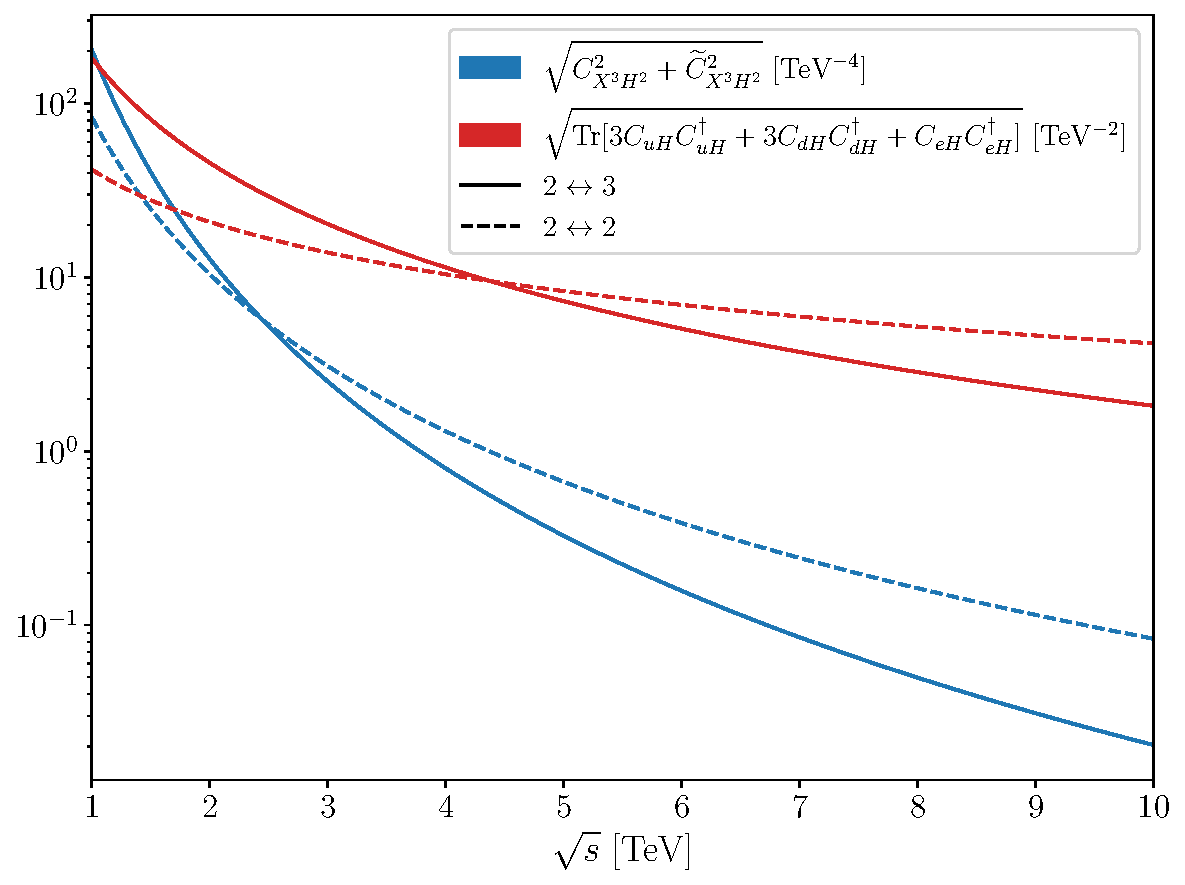
\includegraphics[width=0.8\textwidth]{images/SMEFT_plot_lin.pdf}
\caption{Partial-wave unitarity bounds on the Wilson coefficients of dimension-six (Eq.~\eqref{eq:SMEFT_6}) and dimension-eight (Eq.~\eqref{eq:SMEFT_8}) SMEFT operators
as functions of the center-of-mass energy $\sqrt{s}$ and stemming from
$2\to 2$ processes (dashed lines) and $2\to 3$ processes (solid lines).
$C_{X^3H^2}$ and $\widetilde C_{X^3H^2}$ refer to the gauge group $G=SU(3)$.}
\label{SMEFT_plot}
\end{figure}

\subsection{Dimension-Eight Example}

Next, we consider the following dimension-eight SMEFT interactions~\cite{Murphy:2020rsh}
%
\begin{align}
    \mathcal L^{(8)} \supset C_{X^3H^2}\left(H^\dagger H\right)f^{ABC}X^A_{\mu}{}^{\nu} X^B_{\nu}{}^{\rho} X^C_{\rho}{}^{\mu} + \widetilde C_{X^3H^2}\left(H^\dagger H\right)f^{ABC}X^A_{\mu}{}^{\nu} X^B_{\nu}{}^{\rho} \widetilde X^C_{\rho}{}^{\mu}\,,
    \label{eq:SMEFT_8}
\end{align}
%
where $X^A_{\mu\nu}$ is the field-strength tensor associated with a generic non-Abelian gauge group $G$ and $\widetilde X^A_{\mu\nu} = \frac{1}{2}\epsilon_{\mu\nu\rho\sigma}X^{A}{}^{\rho\sigma}$ is its dual.
%
The strongest unitarity constraint stems from the $J=0$ partial waves and reads
%
\begin{equation}
    C_{X^3H^2}^2+\widetilde C_{X^3H^2}^2 \le
    \left(\frac{32 \sqrt{10} \pi^2}{s^2}\right)^2 \frac{1}{C_2(G)\, d(G)}\,, 
    \label{eq:dim8unbroken}
\end{equation}
%
where $C_2(G)$ is the quadratic Casimir of the adjoint representation of $G$ and $d(G)$ is its dimension.\footnote{$C_2(G)$ is defined by $f^{ACD}f^{BCD} = C_2(G)\delta^{AB}$.
In particular, the structure constants of the $SU(N)$ group, which has dimension 
$d(SU(N)) = N^2 -1$, are normalized such that $C_2(SU(N)) = N$.}
This bound is obtained via a coupled-channel analysis that includes all the processes $\phi_a \phi_b \to X^A{}^\pm X^B{}^\pm X^C{}^\pm$. 
%
Taking the related amplitudes 
%
\begin{align}
    \ket{\mathcal A_{1_{\phi_a},2_{\phi_b} \to 3_{X^A}^-,4_{X^B}^-,5_{X^C}^-}} &= 
    3\sqrt{2}\left(iC_{X^3H^2}-\widetilde C_{X^3H^2}\right)\delta_{ab}  f^{ABC} \agl{3}{4}\agl{4}{5}\agl{3}{5}\,, \\
    \ket{\mathcal A_{1_{\phi_a},2_{\phi_b} \to 3_{X^A}^+,4_{X^B}^+,5_{X^C}^+}} &= 
    3\sqrt{2}\left(iC_{X^3H^2}+\widetilde C_{X^3H^2}\right)\delta_{ab}  f^{ABC} \sqr{4}{3}\sqr{5}{4}\sqr{5}{3}\,,
\end{align}
%
and the relevant vector basis element of Appendix \ref{app:2-to-3_basis}
%
\begin{equation}
    \ket{\mathcal B^0_{1^0,2^0 \to 3^1,4^{1},5^{1}}} = \frac{64\sqrt{30}\pi^2}{s^2}\sqr{4}{3}\sqr{5}{3}\sqr{5}{4}\,,
\end{equation}
%
we can immediately obtain the partial-wave coefficients by including the $1/\sqrt{2}$ symmetry factor:
\begin{align}
    a^0_{1_{\phi_a},2_{\phi_b} \to 
    3_{X^{A}}^\pm,4_{X^{B}}^\pm,5_{X^{C}}^\pm} =
    \frac{3 s^2 }{64\sqrt{30}\pi^2}\delta_{ab}f^{ABC}\left(iC_{X^3H^2}\pm \widetilde C_{X^3H^2}\right)
    \,.
\end{align}

Instead, $h X^A{}^\mp \to X^B{}^\pm X^C{}^\pm$ (corresponding to $J=1$) are the only available $2\to 2$ channels, and the related unitarity bound is
%
\begin{equation}
    C_{X^3H^2}^2+\widetilde C_{X^3H^2}^2 \le 
    %\left(\frac{8\sqrt{2}\pi}{v s^{3/2}}\right)^2 
    \frac{128\pi^2}{s^3 v^2}
    \frac{1}{C_2(G)}\,,
\end{equation}
which is weaker than that of Eq.~\eqref{eq:dim8unbroken} for $\sqrt{s} > 4\pi v\sqrt{5/d(G)}$.

In Figure~\ref{SMEFT_plot}, we show the unitarity bounds 
arising from $2\to 2$ and $2\to 3$ scattering processes as induced 
by $\mathcal L^{(6)}$ and $\mathcal L^{(8)}$; see 
Eqs.~\eqref{eq:SMEFT_6} and \eqref{eq:SMEFT_8}.

\section{Conclusions}

\begin{subappendices}
\section{\texorpdfstring{Angular-Momentum Basis for $2 \to 3$ Amplitudes}{Angular-Momentum Basis for 2-to-3 Amplitudes}\label{app:2-to-3_basis}}

In this appendix we list the normalized kinematic polynomials with definite angular momentum $J_{12}$ relevant for $2 \to 3$ helicity amplitudes, obtained by following the algorithm presented in Section~\ref{sec:PWUB_formalism}.
They are denoted by $\ket*{\mathcal B^{J_{12}}_{i\to f}}$, where $i=(1^{-h_1},2^{-h_2})$ and $f=(3^{h_3},4^{h_4},5^{h_5})$, while $s_{12} = (p_1+p_2)^2$.
They are reported in Table~\ref{tab:2to3basis}.
We report only those with $\sum_{i=1}^5 h_i \ge 0$. The helicity configurations not listed here can be recovered from those reported
by applying a parity flip, i.e., by performing the following substitutions: $h_i \to -h_i$ and $\agl{i}{j}\leftrightarrow \sqr{j}{i}$ for all $i,j$.
Notice that, in many cases, the reported subspace of $V_{i\to f}$ with fixed angular momentum is degenerate.
This degeneracy is due to the fact that a subset of particles in the final state can have more than one angular momentum value.

\begin{comment}
\begin{eqnarray*}
    %\toprule
    \toprule
    (h_1,h_2;h_3,h_4,h_5) &
    %\,\,\,\,\, 
    \qquad\qquad
    J_{12}
    %\,\,\,\,\, 
    \qquad\qquad
    & \ket*{\mathcal B^{J_{12}}_{i \to f}}\\ 
    %\midrule
    \midrule
    (-1,-1;0,1,1) & 0 & 64\sqrt{3}\pi^2s_{12}^{-5/2} \agl{1}{2}^2 \sqr{5}{4}^2 \\
    (-1,-1;\hf,\hf,1) & 0 & 64\sqrt{6}\pi^2s_{12}^{-5/2} \agl{1}{2}^2 \sqr{5}{3}\sqr{5}{4} \\
    (-1,-1;1,1,1) & 0 & 64\sqrt{30}\pi^2s_{12}^{-3} \agl{1}{2}^2 \sqr{4}{3}\sqr{5}{3} \sqr{5}{4} \\
    \hline
    (-1,-\hf;-\hf,1,1) & \hf & 64\sqrt{30}\pi^2s_{12}^{-5/2} \agl{1}{2}\agl{1}{3}\sqr{5}{4}^2 \\
    (-1,-\hf;0,\hf,1) & \hf & 64\sqrt{15}\pi^2s_{12}^{-5/2} \agl{1}{2}\agl{1}{4}\sqr{5}{4}^2 \\
    && 128\sqrt{10}\pi^2s_{12}^{-5/2} \agl{1}{2}\agl{1}{3}\sqr{5}{3}\sqr{5}{4} \\
    (-1,-\hf;\hf,\hf,\hf) & \hf & 64\sqrt{30}\pi^2s_{12}^{-5/2} \agl{1}{2}\agl{1}{3}\sqr{4}{3}\sqr{5}{3} \\
    && 64\sqrt{30}\pi^2s_{12}^{-5/2} \agl{1}{2}\agl{1}{4}\sqr{4}{3}\sqr{5}{4} \\
    && 64\sqrt{30}\pi^2s_{12}^{-5/2} \agl{1}{2}\agl{1}{5}\sqr{5}{3}\sqr{5}{4} \\
    (-1,-\hf;\hf,1,1) & \hf & 384\sqrt{2}\pi^2s_{12}^{-3} \agl{1}{2}\agl{1}{4}\sqr{4}{3}\sqr{5}{4}^2 \\
    && 384\sqrt{2}\pi^2s_{12}^{-3} \agl{1}{2}\agl{1}{5}\sqr{5}{3}\sqr{5}{4}^2 \\
    && 384\sqrt{5}\pi^2s_{12}^{-3} \agl{1}{2}\agl{1}{3}\sqr{4}{3}\sqr{5}{3}\sqr{5}{4} \\
    \hline
    (-1,0;-1,1,1) & 1 & 192\sqrt{15}\pi^2 s_{12}^{-5/2}\agl{1}{3}^2 \sqr{5}{4}^2\\
    (-1,0;-\hf,\hf,1) & 1 & 192\sqrt{15}\pi^2 s_{12}^{-5/2}\agl{1}{3}^2 \sqr{5}{3} \sqr{5}{4} \\
    && 192\sqrt{15}\pi^2 s_{12}^{-5/2}\agl{1}{3}\agl{1}{4} \sqr{5}{4}^2 \\
    (-1,0;0,0,1) & 1 & 288\sqrt{2}\pi^2s_{12}^{-5/2}\agl{1}{4}^2\sqr{5}{4}^2  \\
    && 288\sqrt{2}\pi^2s_{12}^{-5/2}\agl{1}{3}^2\sqr{5}{3}^2 \\
    && 1152\sqrt{\tfrac{5}{7}}\pi^2s_{12}^{-5/2}\agl{1}{3}\agl{1}{4}\sqr{5}{3}\sqr{5}{4} \\
    (-1,0;0,\hf,\hf) & 1 & 576\pi^2 s_{12}^{-5/2}\agl{1}{4}\agl{1}{5}\sqr{5}{4}^2 \\
    && 576\pi^2 s_{12}^{-5/2}\agl{1}{3}^2\sqr{4}{3}\sqr{5}{3} \\
    && 288\sqrt{10}\pi^2 s_{12}^{-5/2}\agl{1}{3}\agl{1}{5}\sqr{5}{3}\sqr{5}{4} \\
    && 288\sqrt{10}\pi^2 s_{12}^{-5/2}\agl{1}{3}\agl{1}{4}\sqr{4}{3}\sqr{5}{4} \\
    (-1,0;0,1,1) & 1 & 192\sqrt{14}\pi^2s_{12}^{-3}\agl{1}{4}\agl{1}{5}\sqr{5}{4}^3 \\
    && 576\sqrt{7}\pi^2s_{12}^{-3}\agl{1}{3}\agl{1}{5}\sqr{5}{3}\sqr{5}{4}^2 \\
    && 576\sqrt{7}\pi^2s_{12}^{-3}\agl{1}{3}\agl{1}{4}\sqr{4}{3}\sqr{5}{4}^2 \\
    && 576\sqrt{7}\pi^2s_{12}^{-3}\agl{1}{3}^2\sqr{4}{3}\sqr{5}{3}\sqr{5}{4} \\
    (-1,0;\hf,\hf,1) & 1 & 192\sqrt{21}\pi^2s_{12}^{-3}\agl{1}{4}^2\sqr{4}{3}\sqr{5}{4}^2 \\
    && 192\sqrt{21}\pi^2s_{12}^{-3}\agl{1}{3}^2\sqr{4}{3}\sqr{5}{3}^2 \\
    && 1152\sqrt{\tfrac{7}{5}}\pi^2s_{12}^{-3}\agl{1}{4}\agl{1}{5}\sqr{5}{3}\sqr{5}{4}^2\\
    && 1152\sqrt{\tfrac{7}{5}}\pi^2s_{12}^{-3}\agl{1}{3}\agl{1}{5}\sqr{5}{3}^2\sqr{5}{4} \\
    && 1152\sqrt{\tfrac{35}{11}}\pi^2s_{12}^{-3}\agl{1}{3}\agl{1}{4}\sqr{4}{3}\sqr{5}{3}\sqr{5}{4} \\
    (-1,0;1,1,1) & 1 & 384\sqrt{15}\pi^2s_{12}^{-7/2} \agl{1}{5}^2\sqr{5}{3}^2 \sqr{5}{4}^2 \\
    && 384\sqrt{15}\pi^2s_{12}^{-7/2} \agl{1}{4}^2\sqr{4}{3}^2 \sqr{5}{4}^2 \\
    && 384\sqrt{15}\pi^2s_{12}^{-7/2} \agl{1}{3}^2\sqr{4}{3}^2 \sqr{5}{3}^2 \\
    && 576\sqrt{35}\pi^2s_{12}^{-7/2} \agl{1}{4}\agl{1}{5}\sqr{4}{3} \sqr{5}{3}\sqr{5}{4}^2 \\
    && 576\sqrt{35}\pi^2s_{12}^{-7/2} \agl{1}{3}\agl{1}{5}\sqr{4}{3} \sqr{5}{3}^2\sqr{5}{4} \\
    && 576\sqrt{35}\pi^2s_{12}^{-7/2} \agl{1}{3}\agl{1}{4}\sqr{4}{3}^2 \sqr{5}{3}\sqr{5}{4} \\
    \hline
    (-1,\hf;-1,\hf,1) & \tfrac{3}{2} & 768\pi^2s_{12}^{-5/2} \agl{1}{3}^2\sqr{5}{2}\sqr{5}{4} \\
    (-1,\hf;-\hf,0,1) & \tfrac{3}{2} & 768\sqrt{\tfrac{15}{37}}\pi^2s_{12}^{-5/2} \agl{1}{3}^2\sqr{5}{2}\sqr{5}{3} \\
    && 768\sqrt{\tfrac{15}{13}}\pi^2s_{12}^{-5/2} \agl{1}{3}\agl{1}{4}\sqr{5}{2}\sqr{5}{4} \\
    (-1,\hf;-\hf,\hf,\hf) & \tfrac{3}{2} & 384\sqrt{3}\pi^2s_{12}^{-5/2} \agl{1}{3}^2\sqr{4}{2}\sqr{5}{3} \\
    && 192\sqrt{30}\pi^2s_{12}^{-5/2} \agl{1}{3}\agl{1}{5}\sqr{5}{2}\sqr{5}{4} \\
    && 192\sqrt{30}\pi^2s_{12}^{-5/2} \agl{1}{3}\agl{1}{4}\sqr{4}{2}\sqr{5}{4} \\
    (-1,\hf;-\hf,1,1) & \tfrac{3}{2} & 768\sqrt{\tfrac{21}{5}}\pi^2s_{12}^{-3} \agl{1}{3}^2\sqr{4}{2}\sqr{5}{3}\sqr{5}{4} \\
    && 768\sqrt{\tfrac{21}{5}}\pi^2s_{12}^{-3} \agl{1}{3}\agl{1}{5}\sqr{5}{2}\sqr{5}{4}^2 \\
    && 768\sqrt{\tfrac{21}{5}}\pi^2s_{12}^{-3} \agl{1}{3}\agl{1}{4}\sqr{4}{2}\sqr{5}{4}^2 \\
    (-1,\hf;0,0,\hf) & \tfrac{3}{2} & 768\pi^2s_{12}^{-5/2} \agl{1}{4}^2\sqr{4}{2}\sqr{5}{4} \\
    && 768\sqrt{\tfrac{15}{13}}\pi^2s_{12}^{-5/2} \agl{1}{3}\agl{1}{5}\sqr{5}{2}\sqr{5}{3} \\
    && 768\sqrt{\tfrac{15}{13}}\pi^2s_{12}^{-5/2} \agl{1}{4}\agl{1}{5}\sqr{5}{2}\sqr{5}{4} \\
    && 384\sqrt{10}\pi^2s_{12}^{-5/2} \agl{1}{3}\agl{1}{4}\sqr{4}{2}\sqr{5}{3} \\
    (-1,\hf;0,\hf,1) & \tfrac{3}{2} & 384\sqrt{7}\pi^2s_{12}^{-3} \agl{1}{3}^2\sqr{4}{2}\sqr{5}{3}^2 \\
    && 384\sqrt{7}\pi^2s_{12}^{-3} \agl{1}{4}^2\sqr{4}{2}\sqr{5}{4}^2 \\
    && 768\sqrt{\tfrac{21}{11}}\pi^2s_{12}^{-3} \agl{1}{4}\agl{1}{5}\sqr{5}{2}\sqr{5}{4}^2 \\
    && 384\sqrt{21}\pi^2s_{12}^{-3} \agl{1}{3}\agl{1}{5}\sqr{5}{2}\sqr{5}{3}\sqr{5}{4} \\
    && 768\sqrt{\tfrac{105}{11}}\pi^2s_{12}^{-3} \agl{1}{3}\agl{1}{4}\sqr{4}{2}\sqr{5}{3}\sqr{5}{4} \\
    (-1,\hf;\hf,\hf,\hf) & \tfrac{3}{2} & 384\sqrt{14}\pi^2s_{12}^{-3} \agl{1}{4}^2\sqr{4}{2}\sqr{4}{3}\sqr{5}{4} \\
    && 384\sqrt{14}\pi^2s_{12}^{-3} \agl{1}{5}^2\sqr{5}{2}\sqr{5}{3}\sqr{5}{4} \\
    && 384\sqrt{14}\pi^2s_{12}^{-3} \agl{1}{3}\agl{1}{5}\sqr{4}{2}\sqr{5}{3}^2 \\
    && 384\sqrt{14}\pi^2s_{12}^{-3} \agl{1}{4}\agl{1}{5}\sqr{3}{2}\sqr{5}{4}^2 \\
    && 192\sqrt{105}\pi^2s_{12}^{-3} \agl{1}{3}\agl{1}{4}\sqr{4}{2}\sqr{4}{3}\sqr{5}{3} \\
    && 192\sqrt{105}\pi^2s_{12}^{-3} \agl{1}{4}\agl{1}{5}\sqr{4}{2}\sqr{5}{3}\sqr{5}{4} \\
    (-1,\hf;\hf,1,1) & \tfrac{3}{2} & 512\sqrt{\tfrac{210}{17}}\pi^2s_{12}^{-7/2} \agl{1}{3}^2\sqr{4}{2}\sqr{4}{3}\sqr{5}{3}^2 \\
    && 512\sqrt{15}\pi^2s_{12}^{-7/2} \agl{1}{4}\agl{1}{5}\sqr{3}{2}\sqr{5}{4}^3 \\
    && 1536\sqrt{2}\pi^2s_{12}^{-7/2} \agl{1}{5}^2\sqr{5}{2}\sqr{5}{3}\sqr{5}{4}^2 \\
    && 1536\sqrt{2}\pi^2s_{12}^{-7/2} \agl{1}{4}^2\sqr{4}{2}\sqr{4}{3}\sqr{5}{4}^2 \\
    && 1536\sqrt{\tfrac{42}{13}}\pi^2s_{12}^{-7/2} \agl{1}{4}\agl{1}{5}\sqr{4}{2}\sqr{5}{3}\sqr{5}{4}^2 \\
    && 1536\sqrt{\tfrac{70}{19}}\pi^2s_{12}^{-7/2} \agl{1}{3}\agl{1}{5}\sqr{4}{2}\sqr{5}{3}^2\sqr{5}{4} \\
    && 1536\sqrt{\tfrac{42}{5}}\pi^2s_{12}^{-7/2} \agl{1}{3}\agl{1}{4}\sqr{4}{2}\sqr{4}{3}\sqr{5}{3}\sqr{5}{4}\\
    \hline
    (-1,1;-1,0,1) & 2 & 96\sqrt{30}\pi^2s_{12}^{-5/2} \agl{1}{3}^2\sqr{5}{2}^2 \\
    (-1,1;-1,\hf,\hf) & 2 & 192\sqrt{15}\pi^2s_{12}^{-5/2} \agl{1}{3}^2\sqr{4}{2}\sqr{5}{2} \\
    (-1,1;-1,1,1) & 2 & 192\sqrt{70}\pi^2s_{12}^{-3} \agl{1}{3}^2\sqr{4}{2}\sqr{5}{2}\sqr{5}{4} \\
    (-1,1;-\hf,0,\hf) & 2 & 960\pi^2s_{12}^{-5/2} \agl{1}{3}\agl{1}{5}\sqr{5}{2}^2 \\
    && 480\sqrt{6}\pi^2s_{12}^{-5/2} \agl{1}{3}\agl{1}{4}\sqr{4}{2}\sqr{5}{2} \\
    (-1,1;-\hf,\hf,1) & 2 & 384\sqrt{\tfrac{105}{11}}\pi^2s_{12}^{-3} \agl{1}{3}^2\sqr{4}{2}\sqr{5}{2}\sqr{5}{3} \\
    && 384\sqrt{21}\pi^2s_{12}^{-3} \agl{1}{3}\agl{1}{5}\sqr{5}{2}^2\sqr{5}{4} \\
    && 192\sqrt{105}\pi^2s_{12}^{-3} \agl{1}{3}\agl{1}{4}\sqr{4}{2}\sqr{5}{2}\sqr{5}{4} \\
    (-1,1;0,0,0) & 2 & 960\pi^2s_{12}^{-5/2} \agl{1}{5}^2\sqr{5}{2}^2 \\
    && 960\pi^2s_{12}^{-5/2} \agl{1}{4}^2\sqr{4}{2}^2 \\
    && 1920\sqrt{\tfrac{3}{7}}\pi^2s_{12}^{-5/2} \agl{1}{4}\agl{1}{5}\sqr{4}{2}\sqr{5}{2} \\
    (-1,1;0,0,1) & 2 & 960\sqrt{\tfrac{21}{11}}\pi^2s_{12}^{-3} \agl{1}{3}\agl{1}{5}\sqr{5}{2}^2\sqr{5}{3} \\
    && 960\sqrt{\tfrac{21}{11}}\pi^2s_{12}^{-3} \agl{1}{4}\agl{1}{5}\sqr{5}{2}^2\sqr{5}{4} \\
    && 960\sqrt{\tfrac{21}{11}}\pi^2s_{12}^{-3} \agl{1}{4}^2\sqr{4}{2}\sqr{5}{2}\sqr{5}{4} \\
    && 480\sqrt{21}\pi^2s_{12}^{-3} \agl{1}{3}\agl{1}{4}\sqr{4}{2}\sqr{5}{2}\sqr{5}{3} \\
    (-1,1;0,\hf,\hf) & 2 & 320\sqrt{21}\pi^2s_{12}^{-3} \agl{1}{5}^2\sqr{5}{2}^2\sqr{5}{4} \\
    && 320\sqrt{21}\pi^2s_{12}^{-3} \agl{1}{4}^2\sqr{4}{2}^2\sqr{5}{4} \\
    && 384\sqrt{35}\pi^2s_{12}^{-3} \agl{1}{3}\agl{1}{4}\sqr{4}{2}^2\sqr{5}{3} \\
    && 192\sqrt{105}\pi^2s_{12}^{-3} \agl{1}{3}\agl{1}{5}\sqr{4}{2}\sqr{5}{2}\sqr{5}{3} \\
    && 640\sqrt{7}\pi^2s_{12}^{-3} \agl{1}{4}\agl{1}{5}\sqr{4}{2}\sqr{5}{2}\sqr{5}{4} \\
    (-1,1;0,1,1) & 2 & 1920\pi^2s_{12}^{-7/2} \agl{1}{3}^2\sqr{4}{2}^2\sqr{5}{3}^2 \\
    && 1920\pi^2s_{12}^{-7/2} \agl{1}{5}^2\sqr{5}{2}^2\sqr{5}{4}^2 \\
    && 1920\pi^2s_{12}^{-7/2} \agl{1}{4}^2\sqr{4}{2}^2\sqr{5}{4}^2 \\
    && 960\sqrt{21}\pi^2s_{12}^{-7/2} \agl{1}{3}\agl{1}{4}\sqr{4}{2}^2\sqr{5}{3}\sqr{5}{4}\\
    && 384\sqrt{30}\pi^2s_{12}^{-7/2} \agl{1}{4}\agl{1}{5}\sqr{4}{2}\sqr{5}{2}\sqr{5}{4}^2 \\
    && 1920\sqrt{\tfrac{42}{11}}\pi^2s_{12}^{-7/2} \agl{1}{3}\agl{1}{5}\sqr{4}{2}\sqr{5}{2}\sqr{5}{3}\sqr{5}{4} \\
    (-1,1;\hf,\hf,1) & 2 & 640\sqrt{42}\pi^2s_{12}^{-7/2} \agl{1}{3}\agl{1}{4}\sqr{4}{2}^2\sqr{5}{3}^2 \\
    && 640\sqrt{42}\pi^2s_{12}^{-7/2} \agl{1}{4}^2\sqr{4}{2}^2\sqr{5}{3}\sqr{5}{4} \\
    && 256\sqrt{105}\pi^2s_{12}^{-7/2} \agl{1}{4}^2\sqr{3}{2}\sqr{4}{2}\sqr{5}{4}^2 \\
    && 1920\sqrt{2}\pi^2s_{12}^{-7/2} \agl{1}{5}^2\sqr{5}{2}^2\sqr{5}{3}\sqr{5}{4} \\
    && 3840\sqrt{\tfrac{7}{13}}\pi^2s_{12}^{-7/2} \agl{1}{3}\agl{1}{5}\sqr{4}{2}\sqr{5}{2}\sqr{5}{3}^2 \\
    && 3840\sqrt{\tfrac{7}{13}}\pi^2s_{12}^{-7/2} \agl{1}{4}\agl{1}{5}\sqr{3}{2}\sqr{5}{2}\sqr{5}{4}^2 \\
    && 3840\sqrt{\tfrac{21}{19}}\pi^2s_{12}^{-7/2} \agl{1}{4}\agl{1}{5}\sqr{4}{2}\sqr{5}{2}\sqr{5}{3}\sqr{5}{4} \\
    (-1,1;1,1,1) & 2 & 288\sqrt{2}\pi^2s_{12}^{-4} \agl{1}{3}\agl{1}{5}\sqr{4}{2}^2\sqr{5}{3}^3 \\
    && 288\sqrt{2}\pi^2s_{12}^{-4} \agl{1}{4}\agl{1}{5}\sqr{3}{2}^2\sqr{5}{4}^3 \\
    && 1152\sqrt{35}\pi^2s_{12}^{-4} \agl{1}{3}\agl{1}{4}\sqr{4}{2}^2\sqr{4}{3}\sqr{5}{3}^2 \\
    && 1152\sqrt{35}\pi^2s_{12}^{-4} \agl{1}{4}\agl{1}{5}\sqr{4}{2}^2\sqr{5}{3}^2\sqr{5}{4} \\
    && 5760\sqrt{2}\pi^2s_{12}^{-4} \agl{1}{4}^2\sqr{4}{2}^2\sqr{4}{3}\sqr{5}{3}\sqr{5}{4} \\
    && 1920\sqrt{6}\pi^2s_{12}^{-4} \agl{1}{4}^2\sqr{3}{2}\sqr{4}{2}\sqr{4}{3}\sqr{5}{4}^2 \\
    && 1920\sqrt{6}\pi^2s_{12}^{-4} \agl{1}{5}^2\sqr{3}{2}\sqr{5}{2}\sqr{5}{3}\sqr{5}{4}^2 \\
    && 1920\sqrt{6}\pi^2s_{12}^{-4} \agl{1}{5}^2\sqr{4}{2}\sqr{5}{2}\sqr{5}{3}^2\sqr{5}{4} \\
    && 960\sqrt{42}\pi^2s_{12}^{-4} \agl{1}{4}\agl{1}{5}\sqr{3}{2}\sqr{4}{2}\sqr{5}{3}\sqr{5}{4}^2 \\
    \hline
    (-\hf,-\hf;-1,1,1) & 1 & 192\sqrt{30}\pi^2s_{12}^{-5/2} \agl{1}{3}\agl{2}{3}\sqr{5}{4}^2 \\
    (-\hf,-\hf;-\hf,\hf,1) & 0 & 64\sqrt{15}\pi^2s_{12}^{-5/2} \agl{1}{2}\agl{3}{4}\sqr{5}{4}^2 \\
    (-\hf,-\hf;0,0,1) & 0 & 64\sqrt{30}\pi^2s_{12}^{-5/2} \agl{1}{2}\agl{3}{4}\sqr{5}{3}\sqr{5}{4} \\
    (-\hf,-\hf;0,\hf,\hf) & 0 & 32\sqrt{6}\pi^2s_{12}^{-3/2} \agl{1}{2}\sqr{5}{4} \\
    (-\hf,-\hf;0,1,1) & 0 & 64\sqrt{3}\pi^2s_{12}^{-2} \agl{1}{2}\sqr{5}{4}^2 \\
    (-\hf,-\hf;\hf,\hf,1) & 0 & 64\sqrt{6}\pi^2s_{12}^{-2} \agl{1}{2}\sqr{5}{3}\sqr{5}{4} \\
    (-\hf,-\hf;1,1,1) & 0 & 64\sqrt{30}\pi^2s_{12}^{-5/2} \agl{1}{2}\sqr{4}{3}\sqr{5}{3}\sqr{5}{4} \\
    \hline
    (-\tfrac{1}{2},0;-1,\tfrac{1}{2},1) & \tfrac{1}{2} & 128\sqrt{30}\pi^2 s_{12}^{-5/2}\agl{1}{3}\agl{3}{4}\sqr{5}{4}^2 \\
    (-\tfrac{1}{2},0;-\tfrac{1}{2},0,1) & \tfrac{1}{2} & 384\sqrt{5}\pi^2 s_{12}^{-5/2} \agl{1}{3}\agl{3}{4}\sqr{5}{3}\sqr{5}{4} \\
    && 128\sqrt{10}\pi^2 s_{12}^{-5/2} \agl{1}{2}\agl{3}{4}\sqr{5}{2}\sqr{5}{4} \\
    (-\tfrac{1}{2},0;-\tfrac{1}{2},\tfrac{1}{2},\tfrac{1}{2}) & \tfrac{1}{2} & 128\sqrt{3}\pi^2 s_{12}^{-3/2}\agl{1}{3}\sqr{5}{4} \\
    (-\tfrac{1}{2},0;-\tfrac{1}{2},1,1) & \tfrac{1}{2} & 64\sqrt{30}\pi^2 s_{12}^{-2}\agl{1}{3}\sqr{5}{4}^2 \\
    (-\tfrac{1}{2},0;0,0,\tfrac{1}{2}) & \tfrac{1}{2} & 128\sqrt{2}\pi^2s_{12}^{-3/2}\agl{1}{3}\sqr{5}{3} \\
    && 128\sqrt{2}\pi^2s_{12}^{-3/2}\agl{1}{4}\sqr{5}{4}\\
    (-\tfrac{1}{2},0;0,\tfrac{1}{2},1) & \tfrac{1}{2} & 64\sqrt{15}\pi^2s_{12}^{-2}\agl{1}{4}\sqr{5}{4}^2 \\
    && 128\sqrt{10}\pi^2 s_{12}^{-2}\agl{1}{3}\sqr{5}{3} \sqr{5}{4} \\
    (-\tfrac{1}{2},0;\tfrac{1}{2},\tfrac{1}{2},\tfrac{1}{2}) & \tfrac{1}{2} & 64\sqrt{30}\pi^2 s_{12}^{-2} \agl{1}{3}\sqr{4}{3}\sqr{5}{3} \\
    && 64\sqrt{30}\pi^2 s_{12}^{-2} \agl{1}{4}\sqr{4}{3}\sqr{5}{4} \\
    && 64\sqrt{30}\pi^2 s_{12}^{-2} \agl{1}{5}\sqr{5}{3}\sqr{5}{4} \\
    (-\tfrac{1}{2},0;\tfrac{1}{2},1,1) & \tfrac{1}{2} & 384\sqrt{5}\pi^2 s_{12}^{-5/2} \agl{1}{3}\sqr{4}{3}\sqr{5}{3}\sqr{5}{4} \\
    && 384\sqrt{5}\pi^2 s_{12}^{-5/2} \agl{1}{4}\sqr{4}{3}\sqr{5}{4}^2 \\
    && 384\sqrt{5}\pi^2 s_{12}^{-5/2} \agl{1}{5}\sqr{5}{3}\sqr{5}{4}^2 \\
    \hline
    (-\hf,\hf;-1,0,1) & 1 & 288\sqrt{10}\pi^2s_{12}^{-5/2} \agl{1}{3}\agl{3}{4}\sqr{5}{2}\sqr{5}{4} \\
    (-\hf,\hf;-1,\hf,\hf) & 1 & 1152\sqrt{\tfrac{5}{13}}\pi^2s_{12}^{-5/2} \agl{1}{3}\agl{3}{5}\sqr{5}{2}\sqr{5}{4} \\
    && 1152\sqrt{\tfrac{5}{13}}\pi^2s_{12}^{-5/2} \agl{1}{3}\agl{3}{4}\sqr{4}{2}\sqr{5}{4} \\
    (-\hf,\hf;-1,1,1) & 1 & 1152\sqrt{\tfrac{35}{31}}\pi^2s_{12}^{-3} \agl{1}{3}\agl{3}{5}\sqr{5}{2}\sqr{5}{4}^2 \\
    && 1152\sqrt{\tfrac{35}{31}}\pi^2s_{12}^{-3} \agl{1}{3}\agl{3}{4}\sqr{4}{2}\sqr{5}{4}^2 \\
    (-\hf,\hf;-\hf,0,\hf) & 1 & 128\sqrt{3}\pi^2s_{12}^{-3/2} \agl{1}{3}\sqr{5}{2} \\
    (-\hf,\hf;-\hf,\hf,1) & 1 & 192\sqrt{5}\pi^2s_{12}^{-2} \agl{1}{3}\sqr{5}{2}\sqr{5}{4} \\
    (-\hf,\hf;0,0,0) & 1 & 192\sqrt{2}\pi^2s_{12}^{-3/2} \agl{1}{4}\sqr{4}{2} \\
    && 192\sqrt{2}\pi^2s_{12}^{-3/2} \agl{1}{5}\sqr{5}{2} \\
    (-\hf,\hf;0,0,1) & 1 & 384\sqrt{\tfrac{5}{7}}\pi^2s_{12}^{-2} \agl{1}{3}\sqr{5}{2}\sqr{5}{3} \\
    && 384\sqrt{\tfrac{5}{7}}\pi^2s_{12}^{-2} \agl{1}{4}\sqr{5}{2}\sqr{5}{4} \\
    (-\hf,\hf;0,\hf,\hf) & 1 & 192\sqrt{5}\pi^2s_{12}^{-2} \agl{1}{3}\sqr{4}{2}\sqr{5}{3} \\
    && 192\sqrt{5}\pi^2s_{12}^{-2} \agl{1}{4}\sqr{4}{2}\sqr{5}{4} \\
    && 192\sqrt{5}\pi^2s_{12}^{-2} \agl{1}{5}\sqr{5}{2}\sqr{5}{4}  \\
    (-\hf,\hf;0,1,1) & 1 & 576\pi^2s_{12}^{-5/2} \agl{1}{5}\sqr{5}{2}\sqr{5}{4}^2  \\
    && 576\pi^2s_{12}^{-5/2} \agl{1}{4}\sqr{4}{2}\sqr{5}{4}^2 \\
    && 288\sqrt{10}\pi^2s_{12}^{-5/2} \agl{1}{3}\sqr{4}{2}\sqr{5}{3}\sqr{5}{4} \\
    (-\hf,\hf;\hf,\hf,1) & 1 & 384\sqrt{3}\pi^2s_{12}^{-5/2} \agl{1}{4}\sqr{3}{2}\sqr{5}{4}^2 \\
    && 384\sqrt{3}\pi^2s_{12}^{-5/2} \agl{1}{3}\sqr{4}{2}\sqr{5}{3}^2 \\
    && 576\sqrt{2}\pi^2s_{12}^{-5/2} \agl{1}{5}\sqr{5}{2}\sqr{5}{3}\sqr{5}{4} \\
    && 192\sqrt{30}\pi^2s_{12}^{-5/2} \agl{1}{4}\sqr{4}{2}\sqr{5}{3}\sqr{5}{4} \\
    (-\hf,\hf;1,1,1) & 1 & 1152\sqrt{\tfrac{35}{31}}\pi^2s_{12}^{-3} \agl{1}{4}\sqr{3}{2}\sqr{4}{3}\sqr{5}{4}^2 \\
    && 1152\sqrt{\tfrac{35}{31}}\pi^2s_{12}^{-3} \agl{1}{5}\sqr{3}{2}\sqr{5}{3}\sqr{5}{4}^2 \\
    && 1152\sqrt{\tfrac{35}{31}}\pi^2s_{12}^{-3} \agl{1}{3}\sqr{4}{2}\sqr{4}{3}\sqr{5}{3}^2 \\
    && 1152\sqrt{\tfrac{35}{31}}\pi^2s_{12}^{-3} \agl{1}{5}\sqr{4}{2}\sqr{5}{3}^2\sqr{5}{4} \\
    && 576\sqrt{14}\pi^2s_{12}^{-3} \agl{1}{4}\sqr{4}{2}\sqr{4}{3}\sqr{5}{3}\sqr{5}{4} \\
    \hline
    (-\hf,1;-1,\hf,1) & \tfrac{3}{2} & 768\sqrt{\tfrac{21}{11}}\pi^2s_{12}^{-3} \agl{1}{3}\agl{3}{5}\sqr{5}{2}^2\sqr{5}{4}\\
    && 384\sqrt{21}\pi^2s_{12}^{-3} \agl{1}{3}\agl{3}{4}\sqr{4}{2}\sqr{5}{2}\sqr{5}{4} \\
    (-\hf,1;-\hf,0,1) & \tfrac{3}{2} & 64\sqrt{30}\pi^2s_{12}^{-2} \agl{1}{3}\sqr{5}{2}^2 \\
    (-\hf,1;-\hf,\hf,\hf) & \tfrac{3}{2} & 128\sqrt{15}\pi^2s_{12}^{-2} \agl{1}{3}\sqr{4}{2}\sqr{5}{2} \\
    (-\hf,1;-\hf,1,1) & \tfrac{3}{2} & 384\sqrt{6}\pi^2s_{12}^{-5/2} \agl{1}{3}\sqr{4}{2}\sqr{5}{2}\sqr{5}{4} \\
    (-\hf,1;0,0,\hf) & \tfrac{3}{2} & 128\sqrt{15}\pi^2s_{12}^{-2} \agl{1}{5}\sqr{5}{2}^2 \\
    && 256\sqrt{5}\pi^2s_{12}^{-2} \agl{1}{4}\sqr{4}{2}\sqr{5}{2} \\
    (-\hf,1;0,\hf,1) & \tfrac{3}{2} & 768\pi^2s_{12}^{-5/2} \agl{1}{5}\sqr{5}{2}^2\sqr{5}{4} \\
    && 768\sqrt{\tfrac{15}{13}}\pi^2s_{12}^{-5/2} \agl{1}{3}\sqr{4}{2}\sqr{5}{2}\sqr{5}{3} \\
    && 768\sqrt{\tfrac{15}{13}}\pi^2s_{12}^{-5/2} \agl{1}{4}\sqr{4}{2}\sqr{5}{2}\sqr{5}{4} \\
    (-\hf,1;\hf,\hf,\hf) & \tfrac{3}{2} & 192\sqrt{30}\pi^2s_{12}^{-5/2} \agl{1}{5}\sqr{4}{2}\sqr{5}{2}\sqr{5}{3} \\
    && 192\sqrt{30}\pi^2s_{12}^{-5/2} \agl{1}{4}\sqr{3}{2}\sqr{4}{2}\sqr{5}{4} \\
    && 192\sqrt{30}\pi^2s_{12}^{-5/2} \agl{1}{5}\sqr{3}{2}\sqr{5}{2}\sqr{5}{4} \\
    && 384\sqrt{10}\pi^2s_{12}^{-5/2} \agl{1}{4}\sqr{4}{2}^2\sqr{5}{3} \\
    (-\hf,1;\hf,1,1) & \tfrac{3}{2} & 128\sqrt{105}\pi^2s_{12}^{-3} \agl{1}{3}\sqr{4}{2}^2\sqr{5}{3}^2 \\
    && 768\sqrt{\tfrac{21}{5}}\pi^2s_{12}^{-3} \agl{1}{4}\sqr{3}{2}\sqr{4}{2}\sqr{5}{4}^2 \\
    && 768\sqrt{\tfrac{21}{5}}\pi^2s_{12}^{-3} \agl{1}{5}\sqr{3}{2}\sqr{5}{2}\sqr{5}{4}^2 \\
    && 768\sqrt{7}\pi^2s_{12}^{-3} \agl{1}{4}\sqr{4}{2}^2\sqr{5}{3}\sqr{5}{4} \\
    && 384\sqrt{21}\pi^2s_{12}^{-3} \agl{1}{5}\sqr{4}{2}\sqr{5}{2}\sqr{5}{3}\sqr{5}{4} \\
    \hline
    (0,0;0,0,0) & 0 & 32\sqrt{2}\pi^2 s_{12}^{-1/2}\\
    (0,0;\tfrac{1}{2},\tfrac{1}{2},0) & 0
    & 32\sqrt{6}\pi^2 s_{12}^{-1}\sqr{4}{3}\\
    (0,0;\tfrac{1}{2},\tfrac{1}{2},1) & 0 & 64\sqrt{6}\pi^2 s_{12}^{-3/2}\sqr{5}{3}\sqr{5}{4}\\
    (0,0;\tfrac{1}{2},\tfrac{1}{2},-1) & 0 & 192\sqrt{10}\pi^2s_{12}^{-5/2}\agl{3}{5}\agl{4}{5}\sqr{4}{3}^2 \\
    (0,0;\tfrac{1}{2},-\tfrac{1}{2},0) & 0 & 64 \sqrt{6}\pi^2 s_{12}^{-3/2}\agl{4}{5}\sqr{5}{3} \\
    (0,0;\tfrac{1}{2},-\tfrac{1}{2},1) & 0 & 64 \sqrt{15}\pi^2s_{12}^{-2}\agl{3}{4}\sqr{5}{3}^2 \\
    (0,0;1,1,0) & 0 & 64\sqrt{3}\pi^2s_{12}^{-3/2}\sqr{4}{3}^2 \\
    (0,0;1,1,1) & 0 & 64\sqrt{30}\pi^2s_{12}^{-2}\sqr{4}{3}\sqr{5}{3}\sqr{5}{4} \\
    (0,0;1,1,-1) & 0 & 64\sqrt{210}\pi^2 s_{12}^{-3}\agl{3}{5}\agl{4}{5}\sqr{4}{3}^3 \\
    (0,0;1,-1,0) & 0 & 192\sqrt{5}\pi^2 s_{12}^{-5/2}\agl{4}{5}^2\sqr{5}{3}^2 \\
    (0,0;1,0,0) & 0 & 64 \sqrt{30}\pi^2s_{12}^{-2}\agl{4}{5}\sqr{4}{3}\sqr{5}{3} \\
    \hline
    (0,\tfrac{1}{2};-1,\tfrac{1}{2},1) & \tfrac{1}{2} & 64\sqrt{210}\pi^2s_{12}^{-3}\agl{3}{4}^2\sqr{4}{2}\sqr{5}{4}^2 \\
    && 128\sqrt{30}\pi^2 s_{12}^{-3}\agl{1}{3}\agl{3}{4}\sqr{2}{1}\sqr{5}{4}^2 \\
    (0,\tfrac{1}{2};-\tfrac{1}{2},0,1) & \tfrac{1}{2} & 128\sqrt{10}\pi^2s_{12}^{-2}\agl{3}{4}\sqr{5}{2}\sqr{5}{4} \\
    (0,\tfrac{1}{2};-\tfrac{1}{2},\tfrac{1}{2},\tfrac{1}{2}) & \tfrac{1}{2} & 64\sqrt{30}\pi^2 s_{12}^{-2} \agl{3}{4}\sqr{4}{2}\sqr{5}{4} \\
    && 128\sqrt{3}\pi^2 s_{12}^{-2}\agl{1}{3}\sqr{2}{1}\sqr{5}{4}\\
    (0,\tfrac{1}{2};-\tfrac{1}{2},1,1) & \tfrac{1}{2} & 384\sqrt{2}\pi^2s_{12}^{-5/2}\agl{3}{4}\sqr{4}{2}\sqr{5}{4}^2 \\
    && 64 \sqrt{30}\pi^2 s_{12}^{-5/2} \agl{1}{3}\sqr{2}{1}\sqr{5}{4}^2\\
    (0,\tfrac{1}{2};0,0,\tfrac{1}{2}) & \tfrac{1}{2} & 64\sqrt{3}\pi^2 s_{12}^{-1}\sqr{5}{2} \\
    (0,\tfrac{1}{2};0,\tfrac{1}{2},1) & \tfrac{1}{2} & 128\sqrt{2}\pi^2s_{12}^{-3/2}\sqr{5}{2}\sqr{5}{4} \\
    (0,\tfrac{1}{2};\tfrac{1}{2},\tfrac{1}{2},\tfrac{1}{2}) & \tfrac{1}{2} & 128\sqrt{3}\pi^2 s_{12}^{-3/2}\sqr{3}{2}\sqr{5}{4} \\
    && 128\sqrt{3}\pi^2 s_{12}^{-3/2}\sqr{4}{3}\sqr{5}{2} \\
    (0,\tfrac{1}{2};\tfrac{1}{2},1,1) & \tfrac{1}{2} & 64\sqrt{30}\pi^2 s_{12}^{-2}\sqr{3}{2}\sqr{5}{4}^2 \\
    && 128\sqrt{10}\pi^2 s_{12}^{-2} \sqr{4}{3}\sqr{5}{2}\sqr{5}{4}\\
    \hline
    (0,1;-1,0,1) & 1 & 576\sqrt{7}\pi^2 s_{12}^{-3}\agl{3}{4}^2\sqr{4}{2}\sqr{5}{2}\sqr{5}{4} \\
    && 576\sqrt{7}\pi^2 s_{12}^{-3}\agl{3}{4}\agl{3}{5}\sqr{5}{2}^2\sqr{5}{4} \\
    (0,1;-1,\hf,\hf) & 1 & 1152\sqrt{\tfrac{35}{11}}\pi^2 s_{12}^{-3}\agl{3}{4}\agl{3}{5}\sqr{4}{2}\sqr{5}{2}\sqr{5}{4} \\
    && 192\sqrt{21}\pi^2 s_{12}^{-3}\agl{3}{5}^2\sqr{5}{2}^2\sqr{5}{4} \\
    && 192\sqrt{21}\pi^2 s_{12}^{-3}\agl{3}{4}^2\sqr{4}{2}^2\sqr{5}{4} \\
    (0,1;-1,1,1) & 1 & 576\sqrt{35}\pi^2 s_{12}^{-7/2} \agl{3}{4}\agl{3}{5}\sqr{4}{2}\sqr{5}{2}\sqr{5}{4}^2 \\
    && 384\sqrt{15}\pi^2 s_{12}^{-7/2} \agl{3}{5}^2\sqr{5}{2}^2\sqr{5}{4}^2 \\
    && 384\sqrt{15}\pi^2 s_{12}^{-7/2} \agl{3}{4}^2\sqr{4}{2}^2\sqr{5}{4}^2 \\
    (0,1;-\hf,-\hf,1) & 1 & 192\sqrt{5}\pi^2 s_{12}^{-2}\agl{3}{4}\sqr{5}{2}^2 \\
    (0,1;-\hf,0,\hf) & 1 & 128\sqrt{15}\pi^2 s_{12}^{-2}\agl{3}{4}\sqr{4}{2}\sqr{5}{2} \\
    && 96\sqrt{10}\pi^2 s_{12}^{-2}\agl{3}{5}\sqr{5}{2}^2 \\
    (0,1;-\hf,\hf,1) & 1 & 576\pi^2 s_{12}^{-5/2}\agl{3}{5}\sqr{5}{2}^2\sqr{5}{4} \\
    && 288\sqrt{10}\pi^2 s_{12}^{-5/2}\agl{3}{4}\sqr{4}{2}\sqr{5}{2}\sqr{5}{4} \\
    (0,1;0,0,0) & 1 & 192\sqrt{5}\pi^2 s_{12}^{-2} \agl{4}{5}\sqr{4}{2}\sqr{5}{2} \\
    && 192\sqrt{5}\pi^2 s_{12}^{-2} \agl{3}{5}\sqr{3}{2}\sqr{5}{2} \\
    && 192\sqrt{5}\pi^2 s_{12}^{-2} \agl{3}{4}\sqr{3}{2}\sqr{4}{2} \\
    (0,1;0,0,1) & 1 & 192\pi^2 s_{12}^{-3/2}\sqr{5}{2}^2 \\
    (0,1;0,\hf,\hf) & 1 & 192\sqrt{2}\pi^2 s_{12}^{-3/2}\sqr{4}{2}\sqr{5}{2} \\
    (0,1;0,1,1) & 1 & 192\sqrt{5}\pi^2 s_{12}^{-2}\sqr{4}{2}\sqr{5}{2}\sqr{5}{4} \\
    (0,1;\hf,\hf,1) & 1 & 128\sqrt{15}\pi^2 s_{12}^{-2}\sqr{4}{2}\sqr{5}{2}\sqr{5}{3} \\
    && 128\sqrt{15}\pi^2 s_{12}^{-2}\sqr{3}{2}\sqr{5}{2}\sqr{5}{4} \\
    (0,1;1,1,1) & 1 & 192\sqrt{15}\pi^2 s_{12}^{-5/2} \sqr{3}{2}^2\sqr{5}{4}^2 \\
    &&  192\sqrt{15}\pi^2 s_{12}^{-5/2} \sqr{4}{2}^2\sqr{5}{3}^2 \\
    &&  1152\sqrt{\tfrac{5}{7}}\pi^2 s_{12}^{-5/2} \sqr{3}{2}\sqr{4}{2}\sqr{5}{3}\sqr{5}{4} \\
    \hline
    (\hf,\hf;-1,0,1) & 0 & 192\sqrt{5}\pi^2 s_{12}^{-3}\agl{3}{4}^2\sqr{2}{1}\sqr{5}{4}^2 \\
    (\hf,\hf;-1,\hf,\hf) & 0 & 192\sqrt{10}\pi^2 s_{12}^{-3}\agl{3}{4}\agl{3}{5}\sqr{2}{1}\sqr{5}{4}^2 \\
    (\hf,\hf;-1,1,1) & 0 & 64\sqrt{210}\pi^2 s_{12}^{-7/2}\agl{3}{4}\agl{3}{5}\sqr{2}{1}\sqr{5}{4}^3 \\
    (\hf,\hf;-\hf,-\hf,1) & 1 & 192\sqrt{10}\pi^2 s_{12}^{-2}\agl{3}{4}\sqr{5}{1}\sqr{5}{2} \\
    (\hf,\hf;-\hf,0,\hf) & 0 & 64\sqrt{6}\pi^2 s_{12}^{-2}\agl{3}{4}\sqr{2}{1}\sqr{5}{4} \\
    (\hf,\hf;-\hf,\hf,1) & 0 & 64\sqrt{15}\pi^2s_{12}^{-5/2}\agl{3}{4}\sqr{2}{1}\sqr{5}{4}^2 \\
    (\hf,\hf;0,0,0) & 0 & 32\sqrt{2}\pi^2 s_{12}^{-1}\sqr{2}{1} \\
    (\hf,\hf;0,0,1) & 1 & 192\sqrt{2}\pi^2s_{12}^{-3/2}\sqr{5}{1}\sqr{5}{2} \\
    (\hf,\hf;0,\hf,\hf) & 0 & 32\sqrt{6}\pi^2 s_{12}^{-3/2}\sqr{2}{1}\sqr{5}{4} \\
    (\hf,\hf;0,1,1) & 0 & 64\sqrt{3}\pi^2 s_{12}^{-2}\sqr{2}{1}\sqr{5}{4}^2 \\
    (\hf,\hf;\hf,\hf,1) & 0 & 64\sqrt{6}\pi^2 s_{12}^{-2}\sqr{2}{1}\sqr{5}{3}\sqr{5}{4} \\
    (\hf,\hf;1,1,1) & 0 & 64\sqrt{30}\pi^2 s_{12}^{-5/2}\sqr{2}{1}\sqr{4}{3}\sqr{5}{3}\sqr{5}{4} \\
    \hline
    (\hf,1;-1,-\hf,1) & \hf & 128\sqrt{30}\pi^2s_{12}^{-3} \agl{3}{4}^2\sqr{2}{1}\sqr{5}{2}\sqr{5}{4} \\
    (\hf,1;-1,0,\hf) & \hf & 384\sqrt{2}\pi^2s_{12}^{-3} \agl{3}{4}^2\sqr{2}{1}\sqr{4}{2}\sqr{5}{4} \\
    && 384\sqrt{5}\pi^2s_{12}^{-3} \agl{3}{4}\agl{3}{5}\sqr{2}{1}\sqr{5}{2}\sqr{5}{4} \\
    (\hf,1;-1,\hf,1) & \hf & 64\sqrt{210}\pi^2s_{12}^{-7/2} \agl{3}{4}^2\sqr{2}{1}\sqr{4}{2}\sqr{5}{4}^2 \\
    && 384\sqrt{14}\pi^2s_{12}^{-7/2} \agl{3}{4}\agl{3}{5}\sqr{2}{1}\sqr{5}{2}\sqr{5}{4}^2 \\
    (\hf,1;-\hf,-\hf,\hf) & \hf & 128\sqrt{3}\pi^2 s_{12}^{-2} \agl{3}{4}\sqr{2}{1}\sqr{5}{2} \\
    (\hf,1;-\hf,0,0) & \hf & 128\sqrt{2}\pi^2 s_{12}^{-2} \agl{3}{4}\sqr{2}{1}\sqr{4}{2} \\
    && 128\sqrt{2} \pi^2s_{12}^{-2} \agl{3}{5}\sqr{2}{1}\sqr{5}{2} \\
    (\hf,1;-\hf,0,1) & \hf & 128\sqrt{10}\pi^2 s_{12}^{-5/2} \agl{3}{4}\sqr{2}{1}\sqr{5}{2}\sqr{5}{4} \\
    (\hf,1;-\hf,\hf,\hf) & \hf & 64\sqrt{30}\pi^2 s_{12}^{-5/2} \agl{3}{4}\sqr{2}{1}\sqr{4}{2}\sqr{5}{4} \\
    && 64\sqrt{30}\pi^2 s_{12}^{-5/2} \agl{3}{5}\sqr{2}{1}\sqr{5}{2}\sqr{5}{4} \\
    (\hf,1;-\hf,1,1) & \hf & 384\sqrt{2}\pi^2 s_{12}^{-3} \agl{3}{4}\sqr{2}{1}\sqr{4}{2}\sqr{5}{4}^2 \\
    && 384\sqrt{2}\pi^2 s_{12}^{-3} \agl{3}{5}\sqr{2}{1}\sqr{5}{2}\sqr{5}{4}^2 \\
    (\hf,1;0,0,\hf) & \hf & 64\sqrt{3}\pi^2 s_{12}^{-3/2} \sqr{2}{1}\sqr{5}{2} \\
    (\hf,1;0,\hf,1) & \hf & 128\sqrt{2}\pi^2 s_{12}^{-2} \sqr{2}{1}\sqr{5}{2}\sqr{5}{4} \\
    (\hf,1;\hf,\hf,\hf) & \hf & 128\sqrt{3}\pi^2 s_{12}^{-2} \sqr{2}{1}\sqr{3}{2}\sqr{5}{4} \\
    && 128\sqrt{3}\pi^2 s_{12}^{-2} \sqr{2}{1}\sqr{4}{2}\sqr{5}{3} \\
    (\hf,1;\hf,1,1) & \hf & 64\sqrt{30}\pi^2 s_{12}^{-5/2} \sqr{2}{1}\sqr{3}{2}\sqr{5}{4}^2 \\
    && 128\sqrt{10}\pi^2 s_{12}^{-5/2} \sqr{2}{1}\sqr{4}{2}\sqr{5}{3}\sqr{5}{4} \\
    \hline
    (1,1;-1,-1,1) & 1 & 192\sqrt{30}\pi^2s_{12}^{-3} \agl{3}{4}^2\sqr{2}{1}\sqr{5}{1}\sqr{5}{2} \\
    (1,1;-1,-\hf,\hf) & 0 & 64\sqrt{15}\pi^2s_{12}^{-3} \agl{3}{4}^2\sqr{2}{1}^2\sqr{5}{4} \\
    (1,1;-1,0,0) & 0 & 64\sqrt{30}\pi^2s_{12}^{-3} \agl{3}{4}\agl{3}{5}\sqr{2}{1}^2\sqr{5}{4} \\
    (1,1;-1,0,1) & 0 & 192\sqrt{5}\pi^2s_{12}^{-7/2} \agl{3}{4}^2\sqr{2}{1}^2\sqr{5}{4}^2 \\
    (1,1;-1,\hf,\hf) & 0 & 192\sqrt{10}\pi^2s_{12}^{-7/2} \agl{3}{4}\agl{3}{5}\sqr{2}{1}^2\sqr{5}{4}^2 \\
    (1,1;-1,1,1) & 0 & 64\sqrt{210}\pi^2s_{12}^{-4} \agl{3}{4}\agl{3}{5}\sqr{2}{1}^2\sqr{5}{4}^3 \\
    (1,1;-\hf,-\hf,0) & 0 & 32\sqrt{6}\pi^2s_{12}^{-2} \agl{3}{4}\sqr{2}{1}^2 \\
    (1,1;-\hf,-\hf,1) & 1 & 192\sqrt{10}\pi^2s_{12}^{-5/2} \agl{3}{4}\sqr{2}{1}\sqr{5}{1}\sqr{5}{2} \\
    (1,1;-\hf,0,\hf) & 0 & 64\sqrt{6}\pi^2s_{12}^{-5/2} \agl{3}{4}\sqr{2}{1}^2\sqr{5}{4} \\
    (1,1;-\hf,\hf,1) & 0 & 64\sqrt{15}\pi^2s_{12}^{-3} \agl{3}{4}\sqr{2}{1}^2 \sqr{5}{4}^2 \\
    (1,1;0,0,0) & 0 &32\sqrt{2}\pi^2s_{12}^{-3/2} \sqr{2}{1}^2 \\
    (1,1;0,0,1) & 1 & 192\sqrt{2}\pi^2s_{12}^{-2} \sqr{2}{1} \sqr{5}{1}\sqr{5}{2} \\
    (1,1;0,\hf,\hf) & 0 & 32\sqrt{6}\pi^2s_{12}^{-2} \sqr{2}{1}^2 \sqr{5}{4} \\
    (1,1;0,1,1) & 0 & 64\sqrt{3}\pi^2s_{12}^{-5/2} \sqr{2}{1}^2 \sqr{5}{4}^2 \\
    (1,1;\hf,\hf,1) & 0 & 64\sqrt{6}\pi^2s_{12}^{-5/2} \sqr{2}{1}^2 \sqr{5}{3}\sqr{5}{4} \\
    (1,1;1,1,1) & 0 & 64\sqrt{30}\pi^2s_{12}^{-3} \sqr{2}{1}^2 \sqr{4}{3}\sqr{5}{3}\sqr{5}{4} \\
    %\bottomrule
    \bottomrule
\end{eqnarray*}
\end{comment}
%% Columns 1-2 auto-wrap in math mode via >{$}c<{$}, so no per-cell $...$
%% needed. Column 3 is left-aligned since several helicity configs expand
%% into a sum of terms, one per row, with cols 1-2 blank on continuations
%% (unchanged from your source).
%%
%% The leading '{}' on the two header rows is NOT a typo -- keep it.
%% booktabs peeks for a literal '(' right after a rule inside a longtable
%% head/foot definition (to support \cmidrule-style trims); since column 1
%% starts with '(', an unguarded header gets its parenthesis silently eaten
%% as a bogus trim spec. '{}' blocks that and is invisible in math mode.
%
\renewcommand{\arraystretch}{1.4}
\begin{longtable}{>{$}l<{$} >{$}c<{$} >{$}l<{$}}
%\caption{[Caption]}\label{tab:2to3basis} \\  % uncomment and fill in if you want one
%\renewcommand{\arraystretch}{1.3}
\toprule
\rowcolor{hdrcolor}
{}(h_1,h_2;h_3,h_4,h_5) & J_{12} & %\multicolumn{1}{c}{$\ket*{\mathcal B^{J_{12}}_{i \to f}}$} \\
\ket*{\mathcal B^{J_{12}}_{i \to f}} \\
\midrule
\endfirsthead
\multicolumn{3}{l}{\small\itshape (continued from previous page)} \\
\toprule
\rowcolor{hdrcolor}
{}(h_1,h_2;h_3,h_4,h_5) & J_{12} & \
%multicolumn{1}{c}{$\ket*{\mathcal B^{J_{12}}_{i \to f}}$} \\
\ket*{\mathcal B^{J_{12}}_{i \to f}} \\
\midrule
\endhead
\midrule
\multicolumn{3}{r}{\small\itshape (continued on next page)} \\
\endfoot
\bottomrule
\caption{Normalized kinematic polynomials $\ket*{\mathcal B^{J_{12}}_{i\to f}}$ for $2 \to 3$ helicity amplitudes with definite angular momentum $J_{12}$. Only helicity configurations with $\sum_{i=1}^5 h_i \ge 0$ are listed; the remaining ones are obtained by parity. Degenerate entries correspond to multiple independent polynomials with the same $J_{12}$.}\label{tab:2to3basis} \\ 
\endlastfoot
    (-1,-1;0,1,1) & 0 & 64\sqrt{3}\pi^2s_{12}^{-5/2} \agl{1}{2}^2 \sqr{5}{4}^2 \\
    (-1,-1;\hf,\hf,1) & 0 & 64\sqrt{6}\pi^2s_{12}^{-5/2} \agl{1}{2}^2 \sqr{5}{3}\sqr{5}{4} \\
    (-1,-1;1,1,1) & 0 & 64\sqrt{30}\pi^2s_{12}^{-3} \agl{1}{2}^2 \sqr{4}{3}\sqr{5}{3} \sqr{5}{4} \\
    \hline
    (-1,-\hf;-\hf,1,1) & \hf & 64\sqrt{30}\pi^2s_{12}^{-5/2} \agl{1}{2}\agl{1}{3}\sqr{5}{4}^2 \\
    (-1,-\hf;0,\hf,1) & \hf & 64\sqrt{15}\pi^2s_{12}^{-5/2} \agl{1}{2}\agl{1}{4}\sqr{5}{4}^2 \\
    && 128\sqrt{10}\pi^2s_{12}^{-5/2} \agl{1}{2}\agl{1}{3}\sqr{5}{3}\sqr{5}{4} \\
    (-1,-\hf;\hf,\hf,\hf) & \hf & 64\sqrt{30}\pi^2s_{12}^{-5/2} \agl{1}{2}\agl{1}{3}\sqr{4}{3}\sqr{5}{3} \\
    && 64\sqrt{30}\pi^2s_{12}^{-5/2} \agl{1}{2}\agl{1}{4}\sqr{4}{3}\sqr{5}{4} \\
    && 64\sqrt{30}\pi^2s_{12}^{-5/2} \agl{1}{2}\agl{1}{5}\sqr{5}{3}\sqr{5}{4} \\
    (-1,-\hf;\hf,1,1) & \hf & 384\sqrt{2}\pi^2s_{12}^{-3} \agl{1}{2}\agl{1}{4}\sqr{4}{3}\sqr{5}{4}^2 \\
    && 384\sqrt{2}\pi^2s_{12}^{-3} \agl{1}{2}\agl{1}{5}\sqr{5}{3}\sqr{5}{4}^2 \\
    && 384\sqrt{5}\pi^2s_{12}^{-3} \agl{1}{2}\agl{1}{3}\sqr{4}{3}\sqr{5}{3}\sqr{5}{4} \\
    \hline
    (-1,0;-1,1,1) & 1 & 192\sqrt{15}\pi^2 s_{12}^{-5/2}\agl{1}{3}^2 \sqr{5}{4}^2\\
    (-1,0;-\hf,\hf,1) & 1 & 192\sqrt{15}\pi^2 s_{12}^{-5/2}\agl{1}{3}^2 \sqr{5}{3} \sqr{5}{4} \\
    && 192\sqrt{15}\pi^2 s_{12}^{-5/2}\agl{1}{3}\agl{1}{4} \sqr{5}{4}^2 \\
    (-1,0;0,0,1) & 1 & 288\sqrt{2}\pi^2s_{12}^{-5/2}\agl{1}{4}^2\sqr{5}{4}^2  \\
    && 288\sqrt{2}\pi^2s_{12}^{-5/2}\agl{1}{3}^2\sqr{5}{3}^2 \\
    && 1152\sqrt{\tfrac{5}{7}}\pi^2s_{12}^{-5/2}\agl{1}{3}\agl{1}{4}\sqr{5}{3}\sqr{5}{4} \\
    (-1,0;0,\hf,\hf) & 1 & 576\pi^2 s_{12}^{-5/2}\agl{1}{4}\agl{1}{5}\sqr{5}{4}^2 \\
    && 576\pi^2 s_{12}^{-5/2}\agl{1}{3}^2\sqr{4}{3}\sqr{5}{3} \\
    && 288\sqrt{10}\pi^2 s_{12}^{-5/2}\agl{1}{3}\agl{1}{5}\sqr{5}{3}\sqr{5}{4} \\
    && 288\sqrt{10}\pi^2 s_{12}^{-5/2}\agl{1}{3}\agl{1}{4}\sqr{4}{3}\sqr{5}{4} \\
    (-1,0;0,1,1) & 1 & 192\sqrt{14}\pi^2s_{12}^{-3}\agl{1}{4}\agl{1}{5}\sqr{5}{4}^3 \\
    && 576\sqrt{7}\pi^2s_{12}^{-3}\agl{1}{3}\agl{1}{5}\sqr{5}{3}\sqr{5}{4}^2 \\
    && 576\sqrt{7}\pi^2s_{12}^{-3}\agl{1}{3}\agl{1}{4}\sqr{4}{3}\sqr{5}{4}^2 \\
    && 576\sqrt{7}\pi^2s_{12}^{-3}\agl{1}{3}^2\sqr{4}{3}\sqr{5}{3}\sqr{5}{4} \\
    (-1,0;\hf,\hf,1) & 1 & 192\sqrt{21}\pi^2s_{12}^{-3}\agl{1}{4}^2\sqr{4}{3}\sqr{5}{4}^2 \\
    && 192\sqrt{21}\pi^2s_{12}^{-3}\agl{1}{3}^2\sqr{4}{3}\sqr{5}{3}^2 \\
    && 1152\sqrt{\tfrac{7}{5}}\pi^2s_{12}^{-3}\agl{1}{4}\agl{1}{5}\sqr{5}{3}\sqr{5}{4}^2\\
    && 1152\sqrt{\tfrac{7}{5}}\pi^2s_{12}^{-3}\agl{1}{3}\agl{1}{5}\sqr{5}{3}^2\sqr{5}{4} \\
    && 1152\sqrt{\tfrac{35}{11}}\pi^2s_{12}^{-3}\agl{1}{3}\agl{1}{4}\sqr{4}{3}\sqr{5}{3}\sqr{5}{4} \\
    (-1,0;1,1,1) & 1 & 384\sqrt{15}\pi^2s_{12}^{-7/2} \agl{1}{5}^2\sqr{5}{3}^2 \sqr{5}{4}^2 \\
    && 384\sqrt{15}\pi^2s_{12}^{-7/2} \agl{1}{4}^2\sqr{4}{3}^2 \sqr{5}{4}^2 \\
    && 384\sqrt{15}\pi^2s_{12}^{-7/2} \agl{1}{3}^2\sqr{4}{3}^2 \sqr{5}{3}^2 \\
    && 576\sqrt{35}\pi^2s_{12}^{-7/2} \agl{1}{4}\agl{1}{5}\sqr{4}{3} \sqr{5}{3}\sqr{5}{4}^2 \\
    && 576\sqrt{35}\pi^2s_{12}^{-7/2} \agl{1}{3}\agl{1}{5}\sqr{4}{3} \sqr{5}{3}^2\sqr{5}{4} \\
    && 576\sqrt{35}\pi^2s_{12}^{-7/2} \agl{1}{3}\agl{1}{4}\sqr{4}{3}^2 \sqr{5}{3}\sqr{5}{4} \\
    \hline
    (-1,\hf;-1,\hf,1) & \tfrac{3}{2} & 768\pi^2s_{12}^{-5/2} \agl{1}{3}^2\sqr{5}{2}\sqr{5}{4} \\
    (-1,\hf;-\hf,0,1) & \tfrac{3}{2} & 768\sqrt{\tfrac{15}{37}}\pi^2s_{12}^{-5/2} \agl{1}{3}^2\sqr{5}{2}\sqr{5}{3} \\
    && 768\sqrt{\tfrac{15}{13}}\pi^2s_{12}^{-5/2} \agl{1}{3}\agl{1}{4}\sqr{5}{2}\sqr{5}{4} \\
    (-1,\hf;-\hf,\hf,\hf) & \tfrac{3}{2} & 384\sqrt{3}\pi^2s_{12}^{-5/2} \agl{1}{3}^2\sqr{4}{2}\sqr{5}{3} \\
    && 192\sqrt{30}\pi^2s_{12}^{-5/2} \agl{1}{3}\agl{1}{5}\sqr{5}{2}\sqr{5}{4} \\
    && 192\sqrt{30}\pi^2s_{12}^{-5/2} \agl{1}{3}\agl{1}{4}\sqr{4}{2}\sqr{5}{4} \\
    (-1,\hf;-\hf,1,1) & \tfrac{3}{2} & 768\sqrt{\tfrac{21}{5}}\pi^2s_{12}^{-3} \agl{1}{3}^2\sqr{4}{2}\sqr{5}{3}\sqr{5}{4} \\
    && 768\sqrt{\tfrac{21}{5}}\pi^2s_{12}^{-3} \agl{1}{3}\agl{1}{5}\sqr{5}{2}\sqr{5}{4}^2 \\
    && 768\sqrt{\tfrac{21}{5}}\pi^2s_{12}^{-3} \agl{1}{3}\agl{1}{4}\sqr{4}{2}\sqr{5}{4}^2 \\
    (-1,\hf;0,0,\hf) & \tfrac{3}{2} & 768\pi^2s_{12}^{-5/2} \agl{1}{4}^2\sqr{4}{2}\sqr{5}{4} \\
    && 768\sqrt{\tfrac{15}{13}}\pi^2s_{12}^{-5/2} \agl{1}{3}\agl{1}{5}\sqr{5}{2}\sqr{5}{3} \\
    && 768\sqrt{\tfrac{15}{13}}\pi^2s_{12}^{-5/2} \agl{1}{4}\agl{1}{5}\sqr{5}{2}\sqr{5}{4} \\
    && 384\sqrt{10}\pi^2s_{12}^{-5/2} \agl{1}{3}\agl{1}{4}\sqr{4}{2}\sqr{5}{3} \\
    (-1,\hf;0,\hf,1) & \tfrac{3}{2} & 384\sqrt{7}\pi^2s_{12}^{-3} \agl{1}{3}^2\sqr{4}{2}\sqr{5}{3}^2 \\
    && 384\sqrt{7}\pi^2s_{12}^{-3} \agl{1}{4}^2\sqr{4}{2}\sqr{5}{4}^2 \\
    && 768\sqrt{\tfrac{21}{11}}\pi^2s_{12}^{-3} \agl{1}{4}\agl{1}{5}\sqr{5}{2}\sqr{5}{4}^2 \\
    && 384\sqrt{21}\pi^2s_{12}^{-3} \agl{1}{3}\agl{1}{5}\sqr{5}{2}\sqr{5}{3}\sqr{5}{4} \\
    && 768\sqrt{\tfrac{105}{11}}\pi^2s_{12}^{-3} \agl{1}{3}\agl{1}{4}\sqr{4}{2}\sqr{5}{3}\sqr{5}{4} \\
    (-1,\hf;\hf,\hf,\hf) & \tfrac{3}{2} & 384\sqrt{14}\pi^2s_{12}^{-3} \agl{1}{4}^2\sqr{4}{2}\sqr{4}{3}\sqr{5}{4} \\
    && 384\sqrt{14}\pi^2s_{12}^{-3} \agl{1}{5}^2\sqr{5}{2}\sqr{5}{3}\sqr{5}{4} \\
    && 384\sqrt{14}\pi^2s_{12}^{-3} \agl{1}{3}\agl{1}{5}\sqr{4}{2}\sqr{5}{3}^2 \\
    && 384\sqrt{14}\pi^2s_{12}^{-3} \agl{1}{4}\agl{1}{5}\sqr{3}{2}\sqr{5}{4}^2 \\
    && 192\sqrt{105}\pi^2s_{12}^{-3} \agl{1}{3}\agl{1}{4}\sqr{4}{2}\sqr{4}{3}\sqr{5}{3} \\
    && 192\sqrt{105}\pi^2s_{12}^{-3} \agl{1}{4}\agl{1}{5}\sqr{4}{2}\sqr{5}{3}\sqr{5}{4} \\
    (-1,\hf;\hf,1,1) & \tfrac{3}{2} & 512\sqrt{\tfrac{210}{17}}\pi^2s_{12}^{-7/2} \agl{1}{3}^2\sqr{4}{2}\sqr{4}{3}\sqr{5}{3}^2 \\
    && 512\sqrt{15}\pi^2s_{12}^{-7/2} \agl{1}{4}\agl{1}{5}\sqr{3}{2}\sqr{5}{4}^3 \\
    && 1536\sqrt{2}\pi^2s_{12}^{-7/2} \agl{1}{5}^2\sqr{5}{2}\sqr{5}{3}\sqr{5}{4}^2 \\
    && 1536\sqrt{2}\pi^2s_{12}^{-7/2} \agl{1}{4}^2\sqr{4}{2}\sqr{4}{3}\sqr{5}{4}^2 \\
    && 1536\sqrt{\tfrac{42}{13}}\pi^2s_{12}^{-7/2} \agl{1}{4}\agl{1}{5}\sqr{4}{2}\sqr{5}{3}\sqr{5}{4}^2 \\
    && 1536\sqrt{\tfrac{70}{19}}\pi^2s_{12}^{-7/2} \agl{1}{3}\agl{1}{5}\sqr{4}{2}\sqr{5}{3}^2\sqr{5}{4} \\
    && 1536\sqrt{\tfrac{42}{5}}\pi^2s_{12}^{-7/2} \agl{1}{3}\agl{1}{4}\sqr{4}{2}\sqr{4}{3}\sqr{5}{3}\sqr{5}{4}\\
    \hline
    (-1,1;-1,0,1) & 2 & 96\sqrt{30}\pi^2s_{12}^{-5/2} \agl{1}{3}^2\sqr{5}{2}^2 \\
    (-1,1;-1,\hf,\hf) & 2 & 192\sqrt{15}\pi^2s_{12}^{-5/2} \agl{1}{3}^2\sqr{4}{2}\sqr{5}{2} \\
    (-1,1;-1,1,1) & 2 & 192\sqrt{70}\pi^2s_{12}^{-3} \agl{1}{3}^2\sqr{4}{2}\sqr{5}{2}\sqr{5}{4} \\
    (-1,1;-\hf,0,\hf) & 2 & 960\pi^2s_{12}^{-5/2} \agl{1}{3}\agl{1}{5}\sqr{5}{2}^2 \\
    && 480\sqrt{6}\pi^2s_{12}^{-5/2} \agl{1}{3}\agl{1}{4}\sqr{4}{2}\sqr{5}{2} \\
    (-1,1;-\hf,\hf,1) & 2 & 384\sqrt{\tfrac{105}{11}}\pi^2s_{12}^{-3} \agl{1}{3}^2\sqr{4}{2}\sqr{5}{2}\sqr{5}{3} \\
    && 384\sqrt{21}\pi^2s_{12}^{-3} \agl{1}{3}\agl{1}{5}\sqr{5}{2}^2\sqr{5}{4} \\
    && 192\sqrt{105}\pi^2s_{12}^{-3} \agl{1}{3}\agl{1}{4}\sqr{4}{2}\sqr{5}{2}\sqr{5}{4} \\
    (-1,1;0,0,0) & 2 & 960\pi^2s_{12}^{-5/2} \agl{1}{5}^2\sqr{5}{2}^2 \\
    && 960\pi^2s_{12}^{-5/2} \agl{1}{4}^2\sqr{4}{2}^2 \\
    && 1920\sqrt{\tfrac{3}{7}}\pi^2s_{12}^{-5/2} \agl{1}{4}\agl{1}{5}\sqr{4}{2}\sqr{5}{2} \\
    (-1,1;0,0,1) & 2 & 960\sqrt{\tfrac{21}{11}}\pi^2s_{12}^{-3} \agl{1}{3}\agl{1}{5}\sqr{5}{2}^2\sqr{5}{3} \\
    && 960\sqrt{\tfrac{21}{11}}\pi^2s_{12}^{-3} \agl{1}{4}\agl{1}{5}\sqr{5}{2}^2\sqr{5}{4} \\
    && 960\sqrt{\tfrac{21}{11}}\pi^2s_{12}^{-3} \agl{1}{4}^2\sqr{4}{2}\sqr{5}{2}\sqr{5}{4} \\
    && 480\sqrt{21}\pi^2s_{12}^{-3} \agl{1}{3}\agl{1}{4}\sqr{4}{2}\sqr{5}{2}\sqr{5}{3} \\
    (-1,1;0,\hf,\hf) & 2 & 320\sqrt{21}\pi^2s_{12}^{-3} \agl{1}{5}^2\sqr{5}{2}^2\sqr{5}{4} \\
    && 320\sqrt{21}\pi^2s_{12}^{-3} \agl{1}{4}^2\sqr{4}{2}^2\sqr{5}{4} \\
    && 384\sqrt{35}\pi^2s_{12}^{-3} \agl{1}{3}\agl{1}{4}\sqr{4}{2}^2\sqr{5}{3} \\
    && 192\sqrt{105}\pi^2s_{12}^{-3} \agl{1}{3}\agl{1}{5}\sqr{4}{2}\sqr{5}{2}\sqr{5}{3} \\
    && 640\sqrt{7}\pi^2s_{12}^{-3} \agl{1}{4}\agl{1}{5}\sqr{4}{2}\sqr{5}{2}\sqr{5}{4} \\
    (-1,1;0,1,1) & 2 & 1920\pi^2s_{12}^{-7/2} \agl{1}{3}^2\sqr{4}{2}^2\sqr{5}{3}^2 \\
    && 1920\pi^2s_{12}^{-7/2} \agl{1}{5}^2\sqr{5}{2}^2\sqr{5}{4}^2 \\
    && 1920\pi^2s_{12}^{-7/2} \agl{1}{4}^2\sqr{4}{2}^2\sqr{5}{4}^2 \\
    && 960\sqrt{21}\pi^2s_{12}^{-7/2} \agl{1}{3}\agl{1}{4}\sqr{4}{2}^2\sqr{5}{3}\sqr{5}{4}\\
    && 384\sqrt{30}\pi^2s_{12}^{-7/2} \agl{1}{4}\agl{1}{5}\sqr{4}{2}\sqr{5}{2}\sqr{5}{4}^2 \\
    && 1920\sqrt{\tfrac{42}{11}}\pi^2s_{12}^{-7/2} \agl{1}{3}\agl{1}{5}\sqr{4}{2}\sqr{5}{2}\sqr{5}{3}\sqr{5}{4} \\
    (-1,1;\hf,\hf,1) & 2 & 640\sqrt{42}\pi^2s_{12}^{-7/2} \agl{1}{3}\agl{1}{4}\sqr{4}{2}^2\sqr{5}{3}^2 \\
    && 640\sqrt{42}\pi^2s_{12}^{-7/2} \agl{1}{4}^2\sqr{4}{2}^2\sqr{5}{3}\sqr{5}{4} \\
    && 256\sqrt{105}\pi^2s_{12}^{-7/2} \agl{1}{4}^2\sqr{3}{2}\sqr{4}{2}\sqr{5}{4}^2 \\
    && 1920\sqrt{2}\pi^2s_{12}^{-7/2} \agl{1}{5}^2\sqr{5}{2}^2\sqr{5}{3}\sqr{5}{4} \\
    && 3840\sqrt{\tfrac{7}{13}}\pi^2s_{12}^{-7/2} \agl{1}{3}\agl{1}{5}\sqr{4}{2}\sqr{5}{2}\sqr{5}{3}^2 \\
    && 3840\sqrt{\tfrac{7}{13}}\pi^2s_{12}^{-7/2} \agl{1}{4}\agl{1}{5}\sqr{3}{2}\sqr{5}{2}\sqr{5}{4}^2 \\
    && 3840\sqrt{\tfrac{21}{19}}\pi^2s_{12}^{-7/2} \agl{1}{4}\agl{1}{5}\sqr{4}{2}\sqr{5}{2}\sqr{5}{3}\sqr{5}{4} \\
    (-1,1;1,1,1) & 2 & 288\sqrt{2}\pi^2s_{12}^{-4} \agl{1}{3}\agl{1}{5}\sqr{4}{2}^2\sqr{5}{3}^3 \\
    && 288\sqrt{2}\pi^2s_{12}^{-4} \agl{1}{4}\agl{1}{5}\sqr{3}{2}^2\sqr{5}{4}^3 \\
    && 1152\sqrt{35}\pi^2s_{12}^{-4} \agl{1}{3}\agl{1}{4}\sqr{4}{2}^2\sqr{4}{3}\sqr{5}{3}^2 \\
    && 1152\sqrt{35}\pi^2s_{12}^{-4} \agl{1}{4}\agl{1}{5}\sqr{4}{2}^2\sqr{5}{3}^2\sqr{5}{4} \\
    && 5760\sqrt{2}\pi^2s_{12}^{-4} \agl{1}{4}^2\sqr{4}{2}^2\sqr{4}{3}\sqr{5}{3}\sqr{5}{4} \\
    && 1920\sqrt{6}\pi^2s_{12}^{-4} \agl{1}{4}^2\sqr{3}{2}\sqr{4}{2}\sqr{4}{3}\sqr{5}{4}^2 \\
    && 1920\sqrt{6}\pi^2s_{12}^{-4} \agl{1}{5}^2\sqr{3}{2}\sqr{5}{2}\sqr{5}{3}\sqr{5}{4}^2 \\
    && 1920\sqrt{6}\pi^2s_{12}^{-4} \agl{1}{5}^2\sqr{4}{2}\sqr{5}{2}\sqr{5}{3}^2\sqr{5}{4} \\
    && 960\sqrt{42}\pi^2s_{12}^{-4} \agl{1}{4}\agl{1}{5}\sqr{3}{2}\sqr{4}{2}\sqr{5}{3}\sqr{5}{4}^2 \\
    \hline
    (-\hf,-\hf;-1,1,1) & 1 & 192\sqrt{30}\pi^2s_{12}^{-5/2} \agl{1}{3}\agl{2}{3}\sqr{5}{4}^2 \\
    (-\hf,-\hf;-\hf,\hf,1) & 0 & 64\sqrt{15}\pi^2s_{12}^{-5/2} \agl{1}{2}\agl{3}{4}\sqr{5}{4}^2 \\
    (-\hf,-\hf;0,0,1) & 0 & 64\sqrt{30}\pi^2s_{12}^{-5/2} \agl{1}{2}\agl{3}{4}\sqr{5}{3}\sqr{5}{4} \\
    (-\hf,-\hf;0,\hf,\hf) & 0 & 32\sqrt{6}\pi^2s_{12}^{-3/2} \agl{1}{2}\sqr{5}{4} \\
    (-\hf,-\hf;0,1,1) & 0 & 64\sqrt{3}\pi^2s_{12}^{-2} \agl{1}{2}\sqr{5}{4}^2 \\
    (-\hf,-\hf;\hf,\hf,1) & 0 & 64\sqrt{6}\pi^2s_{12}^{-2} \agl{1}{2}\sqr{5}{3}\sqr{5}{4} \\
    (-\hf,-\hf;1,1,1) & 0 & 64\sqrt{30}\pi^2s_{12}^{-5/2} \agl{1}{2}\sqr{4}{3}\sqr{5}{3}\sqr{5}{4} \\
    \hline
    (-\tfrac{1}{2},0;-1,\tfrac{1}{2},1) & \tfrac{1}{2} & 128\sqrt{30}\pi^2 s_{12}^{-5/2}\agl{1}{3}\agl{3}{4}\sqr{5}{4}^2 \\
    (-\tfrac{1}{2},0;-\tfrac{1}{2},0,1) & \tfrac{1}{2} & 384\sqrt{5}\pi^2 s_{12}^{-5/2} \agl{1}{3}\agl{3}{4}\sqr{5}{3}\sqr{5}{4} \\
    && 128\sqrt{10}\pi^2 s_{12}^{-5/2} \agl{1}{2}\agl{3}{4}\sqr{5}{2}\sqr{5}{4} \\
    (-\tfrac{1}{2},0;-\tfrac{1}{2},\tfrac{1}{2},\tfrac{1}{2}) & \tfrac{1}{2} & 128\sqrt{3}\pi^2 s_{12}^{-3/2}\agl{1}{3}\sqr{5}{4} \\
    (-\tfrac{1}{2},0;-\tfrac{1}{2},1,1) & \tfrac{1}{2} & 64\sqrt{30}\pi^2 s_{12}^{-2}\agl{1}{3}\sqr{5}{4}^2 \\
    (-\tfrac{1}{2},0;0,0,\tfrac{1}{2}) & \tfrac{1}{2} & 128\sqrt{2}\pi^2s_{12}^{-3/2}\agl{1}{3}\sqr{5}{3} \\
    && 128\sqrt{2}\pi^2s_{12}^{-3/2}\agl{1}{4}\sqr{5}{4}\\
    (-\tfrac{1}{2},0;0,\tfrac{1}{2},1) & \tfrac{1}{2} & 64\sqrt{15}\pi^2s_{12}^{-2}\agl{1}{4}\sqr{5}{4}^2 \\
    && 128\sqrt{10}\pi^2 s_{12}^{-2}\agl{1}{3}\sqr{5}{3} \sqr{5}{4} \\
    (-\tfrac{1}{2},0;\tfrac{1}{2},\tfrac{1}{2},\tfrac{1}{2}) & \tfrac{1}{2} & 64\sqrt{30}\pi^2 s_{12}^{-2} \agl{1}{3}\sqr{4}{3}\sqr{5}{3} \\
    && 64\sqrt{30}\pi^2 s_{12}^{-2} \agl{1}{4}\sqr{4}{3}\sqr{5}{4} \\
    && 64\sqrt{30}\pi^2 s_{12}^{-2} \agl{1}{5}\sqr{5}{3}\sqr{5}{4} \\
    (-\tfrac{1}{2},0;\tfrac{1}{2},1,1) & \tfrac{1}{2} & 384\sqrt{5}\pi^2 s_{12}^{-5/2} \agl{1}{3}\sqr{4}{3}\sqr{5}{3}\sqr{5}{4} \\
    && 384\sqrt{5}\pi^2 s_{12}^{-5/2} \agl{1}{4}\sqr{4}{3}\sqr{5}{4}^2 \\
    && 384\sqrt{5}\pi^2 s_{12}^{-5/2} \agl{1}{5}\sqr{5}{3}\sqr{5}{4}^2 \\
    \hline
    (-\hf,\hf;-1,0,1) & 1 & 288\sqrt{10}\pi^2s_{12}^{-5/2} \agl{1}{3}\agl{3}{4}\sqr{5}{2}\sqr{5}{4} \\
    (-\hf,\hf;-1,\hf,\hf) & 1 & 1152\sqrt{\tfrac{5}{13}}\pi^2s_{12}^{-5/2} \agl{1}{3}\agl{3}{5}\sqr{5}{2}\sqr{5}{4} \\
    && 1152\sqrt{\tfrac{5}{13}}\pi^2s_{12}^{-5/2} \agl{1}{3}\agl{3}{4}\sqr{4}{2}\sqr{5}{4} \\
    (-\hf,\hf;-1,1,1) & 1 & 1152\sqrt{\tfrac{35}{31}}\pi^2s_{12}^{-3} \agl{1}{3}\agl{3}{5}\sqr{5}{2}\sqr{5}{4}^2 \\
    && 1152\sqrt{\tfrac{35}{31}}\pi^2s_{12}^{-3} \agl{1}{3}\agl{3}{4}\sqr{4}{2}\sqr{5}{4}^2 \\
    (-\hf,\hf;-\hf,0,\hf) & 1 & 128\sqrt{3}\pi^2s_{12}^{-3/2} \agl{1}{3}\sqr{5}{2} \\
    (-\hf,\hf;-\hf,\hf,1) & 1 & 192\sqrt{5}\pi^2s_{12}^{-2} \agl{1}{3}\sqr{5}{2}\sqr{5}{4} \\
    (-\hf,\hf;0,0,0) & 1 & 192\sqrt{2}\pi^2s_{12}^{-3/2} \agl{1}{4}\sqr{4}{2} \\
    && 192\sqrt{2}\pi^2s_{12}^{-3/2} \agl{1}{5}\sqr{5}{2} \\
    (-\hf,\hf;0,0,1) & 1 & 384\sqrt{\tfrac{5}{7}}\pi^2s_{12}^{-2} \agl{1}{3}\sqr{5}{2}\sqr{5}{3} \\
    && 384\sqrt{\tfrac{5}{7}}\pi^2s_{12}^{-2} \agl{1}{4}\sqr{5}{2}\sqr{5}{4} \\
    (-\hf,\hf;0,\hf,\hf) & 1 & 192\sqrt{5}\pi^2s_{12}^{-2} \agl{1}{3}\sqr{4}{2}\sqr{5}{3} \\
    && 192\sqrt{5}\pi^2s_{12}^{-2} \agl{1}{4}\sqr{4}{2}\sqr{5}{4} \\
    && 192\sqrt{5}\pi^2s_{12}^{-2} \agl{1}{5}\sqr{5}{2}\sqr{5}{4}  \\
    (-\hf,\hf;0,1,1) & 1 & 576\pi^2s_{12}^{-5/2} \agl{1}{5}\sqr{5}{2}\sqr{5}{4}^2  \\
    && 576\pi^2s_{12}^{-5/2} \agl{1}{4}\sqr{4}{2}\sqr{5}{4}^2 \\
    && 288\sqrt{10}\pi^2s_{12}^{-5/2} \agl{1}{3}\sqr{4}{2}\sqr{5}{3}\sqr{5}{4} \\
    (-\hf,\hf;\hf,\hf,1) & 1 & 384\sqrt{3}\pi^2s_{12}^{-5/2} \agl{1}{4}\sqr{3}{2}\sqr{5}{4}^2 \\
    && 384\sqrt{3}\pi^2s_{12}^{-5/2} \agl{1}{3}\sqr{4}{2}\sqr{5}{3}^2 \\
    && 576\sqrt{2}\pi^2s_{12}^{-5/2} \agl{1}{5}\sqr{5}{2}\sqr{5}{3}\sqr{5}{4} \\
    && 192\sqrt{30}\pi^2s_{12}^{-5/2} \agl{1}{4}\sqr{4}{2}\sqr{5}{3}\sqr{5}{4} \\
    (-\hf,\hf;1,1,1) & 1 & 1152\sqrt{\tfrac{35}{31}}\pi^2s_{12}^{-3} \agl{1}{4}\sqr{3}{2}\sqr{4}{3}\sqr{5}{4}^2 \\
    && 1152\sqrt{\tfrac{35}{31}}\pi^2s_{12}^{-3} \agl{1}{5}\sqr{3}{2}\sqr{5}{3}\sqr{5}{4}^2 \\
    && 1152\sqrt{\tfrac{35}{31}}\pi^2s_{12}^{-3} \agl{1}{3}\sqr{4}{2}\sqr{4}{3}\sqr{5}{3}^2 \\
    && 1152\sqrt{\tfrac{35}{31}}\pi^2s_{12}^{-3} \agl{1}{5}\sqr{4}{2}\sqr{5}{3}^2\sqr{5}{4} \\
    && 576\sqrt{14}\pi^2s_{12}^{-3} \agl{1}{4}\sqr{4}{2}\sqr{4}{3}\sqr{5}{3}\sqr{5}{4} \\
    \hline
    (-\hf,1;-1,\hf,1) & \tfrac{3}{2} & 768\sqrt{\tfrac{21}{11}}\pi^2s_{12}^{-3} \agl{1}{3}\agl{3}{5}\sqr{5}{2}^2\sqr{5}{4}\\
    && 384\sqrt{21}\pi^2s_{12}^{-3} \agl{1}{3}\agl{3}{4}\sqr{4}{2}\sqr{5}{2}\sqr{5}{4} \\
    (-\hf,1;-\hf,0,1) & \tfrac{3}{2} & 64\sqrt{30}\pi^2s_{12}^{-2} \agl{1}{3}\sqr{5}{2}^2 \\
    (-\hf,1;-\hf,\hf,\hf) & \tfrac{3}{2} & 128\sqrt{15}\pi^2s_{12}^{-2} \agl{1}{3}\sqr{4}{2}\sqr{5}{2} \\
    (-\hf,1;-\hf,1,1) & \tfrac{3}{2} & 384\sqrt{6}\pi^2s_{12}^{-5/2} \agl{1}{3}\sqr{4}{2}\sqr{5}{2}\sqr{5}{4} \\
    (-\hf,1;0,0,\hf) & \tfrac{3}{2} & 128\sqrt{15}\pi^2s_{12}^{-2} \agl{1}{5}\sqr{5}{2}^2 \\
    && 256\sqrt{5}\pi^2s_{12}^{-2} \agl{1}{4}\sqr{4}{2}\sqr{5}{2} \\
    (-\hf,1;0,\hf,1) & \tfrac{3}{2} & 768\pi^2s_{12}^{-5/2} \agl{1}{5}\sqr{5}{2}^2\sqr{5}{4} \\
    && 768\sqrt{\tfrac{15}{13}}\pi^2s_{12}^{-5/2} \agl{1}{3}\sqr{4}{2}\sqr{5}{2}\sqr{5}{3} \\
    && 768\sqrt{\tfrac{15}{13}}\pi^2s_{12}^{-5/2} \agl{1}{4}\sqr{4}{2}\sqr{5}{2}\sqr{5}{4} \\
    (-\hf,1;\hf,\hf,\hf) & \tfrac{3}{2} & 192\sqrt{30}\pi^2s_{12}^{-5/2} \agl{1}{5}\sqr{4}{2}\sqr{5}{2}\sqr{5}{3} \\
    && 192\sqrt{30}\pi^2s_{12}^{-5/2} \agl{1}{4}\sqr{3}{2}\sqr{4}{2}\sqr{5}{4} \\
    && 192\sqrt{30}\pi^2s_{12}^{-5/2} \agl{1}{5}\sqr{3}{2}\sqr{5}{2}\sqr{5}{4} \\
    && 384\sqrt{10}\pi^2s_{12}^{-5/2} \agl{1}{4}\sqr{4}{2}^2\sqr{5}{3} \\
    (-\hf,1;\hf,1,1) & \tfrac{3}{2} & 128\sqrt{105}\pi^2s_{12}^{-3} \agl{1}{3}\sqr{4}{2}^2\sqr{5}{3}^2 \\
    && 768\sqrt{\tfrac{21}{5}}\pi^2s_{12}^{-3} \agl{1}{4}\sqr{3}{2}\sqr{4}{2}\sqr{5}{4}^2 \\
    && 768\sqrt{\tfrac{21}{5}}\pi^2s_{12}^{-3} \agl{1}{5}\sqr{3}{2}\sqr{5}{2}\sqr{5}{4}^2 \\
    && 768\sqrt{7}\pi^2s_{12}^{-3} \agl{1}{4}\sqr{4}{2}^2\sqr{5}{3}\sqr{5}{4} \\
    && 384\sqrt{21}\pi^2s_{12}^{-3} \agl{1}{5}\sqr{4}{2}\sqr{5}{2}\sqr{5}{3}\sqr{5}{4} \\
    \hline
    (0,0;0,0,0) & 0 & 32\sqrt{2}\pi^2 s_{12}^{-1/2}\\
    (0,0;\tfrac{1}{2},\tfrac{1}{2},0) & 0
    & 32\sqrt{6}\pi^2 s_{12}^{-1}\sqr{4}{3}\\
    (0,0;\tfrac{1}{2},\tfrac{1}{2},1) & 0 & 64\sqrt{6}\pi^2 s_{12}^{-3/2}\sqr{5}{3}\sqr{5}{4}\\
    (0,0;\tfrac{1}{2},\tfrac{1}{2},-1) & 0 & 192\sqrt{10}\pi^2s_{12}^{-5/2}\agl{3}{5}\agl{4}{5}\sqr{4}{3}^2 \\
    (0,0;\tfrac{1}{2},-\tfrac{1}{2},0) & 0 & 64 \sqrt{6}\pi^2 s_{12}^{-3/2}\agl{4}{5}\sqr{5}{3} \\
    (0,0;\tfrac{1}{2},-\tfrac{1}{2},1) & 0 & 64 \sqrt{15}\pi^2s_{12}^{-2}\agl{3}{4}\sqr{5}{3}^2 \\
    (0,0;1,1,0) & 0 & 64\sqrt{3}\pi^2s_{12}^{-3/2}\sqr{4}{3}^2 \\
    (0,0;1,1,1) & 0 & 64\sqrt{30}\pi^2s_{12}^{-2}\sqr{4}{3}\sqr{5}{3}\sqr{5}{4} \\
    (0,0;1,1,-1) & 0 & 64\sqrt{210}\pi^2 s_{12}^{-3}\agl{3}{5}\agl{4}{5}\sqr{4}{3}^3 \\
    (0,0;1,-1,0) & 0 & 192\sqrt{5}\pi^2 s_{12}^{-5/2}\agl{4}{5}^2\sqr{5}{3}^2 \\
    (0,0;1,0,0) & 0 & 64 \sqrt{30}\pi^2s_{12}^{-2}\agl{4}{5}\sqr{4}{3}\sqr{5}{3} \\
    \hline
    (0,\tfrac{1}{2};-1,\tfrac{1}{2},1) & \tfrac{1}{2} & 64\sqrt{210}\pi^2s_{12}^{-3}\agl{3}{4}^2\sqr{4}{2}\sqr{5}{4}^2 \\
    && 128\sqrt{30}\pi^2 s_{12}^{-3}\agl{1}{3}\agl{3}{4}\sqr{2}{1}\sqr{5}{4}^2 \\
    (0,\tfrac{1}{2};-\tfrac{1}{2},0,1) & \tfrac{1}{2} & 128\sqrt{10}\pi^2s_{12}^{-2}\agl{3}{4}\sqr{5}{2}\sqr{5}{4} \\
    (0,\tfrac{1}{2};-\tfrac{1}{2},\tfrac{1}{2},\tfrac{1}{2}) & \tfrac{1}{2} & 64\sqrt{30}\pi^2 s_{12}^{-2} \agl{3}{4}\sqr{4}{2}\sqr{5}{4} \\
    && 128\sqrt{3}\pi^2 s_{12}^{-2}\agl{1}{3}\sqr{2}{1}\sqr{5}{4}\\
    (0,\tfrac{1}{2};-\tfrac{1}{2},1,1) & \tfrac{1}{2} & 384\sqrt{2}\pi^2s_{12}^{-5/2}\agl{3}{4}\sqr{4}{2}\sqr{5}{4}^2 \\
    && 64 \sqrt{30}\pi^2 s_{12}^{-5/2} \agl{1}{3}\sqr{2}{1}\sqr{5}{4}^2\\
    (0,\tfrac{1}{2};0,0,\tfrac{1}{2}) & \tfrac{1}{2} & 64\sqrt{3}\pi^2 s_{12}^{-1}\sqr{5}{2} \\
    (0,\tfrac{1}{2};0,\tfrac{1}{2},1) & \tfrac{1}{2} & 128\sqrt{2}\pi^2s_{12}^{-3/2}\sqr{5}{2}\sqr{5}{4} \\
    (0,\tfrac{1}{2};\tfrac{1}{2},\tfrac{1}{2},\tfrac{1}{2}) & \tfrac{1}{2} & 128\sqrt{3}\pi^2 s_{12}^{-3/2}\sqr{3}{2}\sqr{5}{4} \\
    && 128\sqrt{3}\pi^2 s_{12}^{-3/2}\sqr{4}{3}\sqr{5}{2} \\
    (0,\tfrac{1}{2};\tfrac{1}{2},1,1) & \tfrac{1}{2} & 64\sqrt{30}\pi^2 s_{12}^{-2}\sqr{3}{2}\sqr{5}{4}^2 \\
    && 128\sqrt{10}\pi^2 s_{12}^{-2} \sqr{4}{3}\sqr{5}{2}\sqr{5}{4}\\
    \hline
    (0,1;-1,0,1) & 1 & 576\sqrt{7}\pi^2 s_{12}^{-3}\agl{3}{4}^2\sqr{4}{2}\sqr{5}{2}\sqr{5}{4} \\
    && 576\sqrt{7}\pi^2 s_{12}^{-3}\agl{3}{4}\agl{3}{5}\sqr{5}{2}^2\sqr{5}{4} \\
    (0,1;-1,\hf,\hf) & 1 & 1152\sqrt{\tfrac{35}{11}}\pi^2 s_{12}^{-3}\agl{3}{4}\agl{3}{5}\sqr{4}{2}\sqr{5}{2}\sqr{5}{4} \\
    && 192\sqrt{21}\pi^2 s_{12}^{-3}\agl{3}{5}^2\sqr{5}{2}^2\sqr{5}{4} \\
    && 192\sqrt{21}\pi^2 s_{12}^{-3}\agl{3}{4}^2\sqr{4}{2}^2\sqr{5}{4} \\
    (0,1;-1,1,1) & 1 & 576\sqrt{35}\pi^2 s_{12}^{-7/2} \agl{3}{4}\agl{3}{5}\sqr{4}{2}\sqr{5}{2}\sqr{5}{4}^2 \\
    && 384\sqrt{15}\pi^2 s_{12}^{-7/2} \agl{3}{5}^2\sqr{5}{2}^2\sqr{5}{4}^2 \\
    && 384\sqrt{15}\pi^2 s_{12}^{-7/2} \agl{3}{4}^2\sqr{4}{2}^2\sqr{5}{4}^2 \\
    (0,1;-\hf,-\hf,1) & 1 & 192\sqrt{5}\pi^2 s_{12}^{-2}\agl{3}{4}\sqr{5}{2}^2 \\
    (0,1;-\hf,0,\hf) & 1 & 128\sqrt{15}\pi^2 s_{12}^{-2}\agl{3}{4}\sqr{4}{2}\sqr{5}{2} \\
    && 96\sqrt{10}\pi^2 s_{12}^{-2}\agl{3}{5}\sqr{5}{2}^2 \\
    (0,1;-\hf,\hf,1) & 1 & 576\pi^2 s_{12}^{-5/2}\agl{3}{5}\sqr{5}{2}^2\sqr{5}{4} \\
    && 288\sqrt{10}\pi^2 s_{12}^{-5/2}\agl{3}{4}\sqr{4}{2}\sqr{5}{2}\sqr{5}{4} \\
    (0,1;0,0,0) & 1 & 192\sqrt{5}\pi^2 s_{12}^{-2} \agl{4}{5}\sqr{4}{2}\sqr{5}{2} \\
    && 192\sqrt{5}\pi^2 s_{12}^{-2} \agl{3}{5}\sqr{3}{2}\sqr{5}{2} \\
    && 192\sqrt{5}\pi^2 s_{12}^{-2} \agl{3}{4}\sqr{3}{2}\sqr{4}{2} \\
    (0,1;0,0,1) & 1 & 192\pi^2 s_{12}^{-3/2}\sqr{5}{2}^2 \\
    (0,1;0,\hf,\hf) & 1 & 192\sqrt{2}\pi^2 s_{12}^{-3/2}\sqr{4}{2}\sqr{5}{2} \\
    (0,1;0,1,1) & 1 & 192\sqrt{5}\pi^2 s_{12}^{-2}\sqr{4}{2}\sqr{5}{2}\sqr{5}{4} \\
    (0,1;\hf,\hf,1) & 1 & 128\sqrt{15}\pi^2 s_{12}^{-2}\sqr{4}{2}\sqr{5}{2}\sqr{5}{3} \\
    && 128\sqrt{15}\pi^2 s_{12}^{-2}\sqr{3}{2}\sqr{5}{2}\sqr{5}{4} \\
    (0,1;1,1,1) & 1 & 192\sqrt{15}\pi^2 s_{12}^{-5/2} \sqr{3}{2}^2\sqr{5}{4}^2 \\
    &&  192\sqrt{15}\pi^2 s_{12}^{-5/2} \sqr{4}{2}^2\sqr{5}{3}^2 \\
    &&  1152\sqrt{\tfrac{5}{7}}\pi^2 s_{12}^{-5/2} \sqr{3}{2}\sqr{4}{2}\sqr{5}{3}\sqr{5}{4} \\
    \hline
    (\hf,\hf;-1,0,1) & 0 & 192\sqrt{5}\pi^2 s_{12}^{-3}\agl{3}{4}^2\sqr{2}{1}\sqr{5}{4}^2 \\
    (\hf,\hf;-1,\hf,\hf) & 0 & 192\sqrt{10}\pi^2 s_{12}^{-3}\agl{3}{4}\agl{3}{5}\sqr{2}{1}\sqr{5}{4}^2 \\
    (\hf,\hf;-1,1,1) & 0 & 64\sqrt{210}\pi^2 s_{12}^{-7/2}\agl{3}{4}\agl{3}{5}\sqr{2}{1}\sqr{5}{4}^3 \\
    (\hf,\hf;-\hf,-\hf,1) & 1 & 192\sqrt{10}\pi^2 s_{12}^{-2}\agl{3}{4}\sqr{5}{1}\sqr{5}{2} \\
    (\hf,\hf;-\hf,0,\hf) & 0 & 64\sqrt{6}\pi^2 s_{12}^{-2}\agl{3}{4}\sqr{2}{1}\sqr{5}{4} \\
    (\hf,\hf;-\hf,\hf,1) & 0 & 64\sqrt{15}\pi^2s_{12}^{-5/2}\agl{3}{4}\sqr{2}{1}\sqr{5}{4}^2 \\
    (\hf,\hf;0,0,0) & 0 & 32\sqrt{2}\pi^2 s_{12}^{-1}\sqr{2}{1} \\
    (\hf,\hf;0,0,1) & 1 & 192\sqrt{2}\pi^2s_{12}^{-3/2}\sqr{5}{1}\sqr{5}{2} \\
    (\hf,\hf;0,\hf,\hf) & 0 & 32\sqrt{6}\pi^2 s_{12}^{-3/2}\sqr{2}{1}\sqr{5}{4} \\
    (\hf,\hf;0,1,1) & 0 & 64\sqrt{3}\pi^2 s_{12}^{-2}\sqr{2}{1}\sqr{5}{4}^2 \\
    (\hf,\hf;\hf,\hf,1) & 0 & 64\sqrt{6}\pi^2 s_{12}^{-2}\sqr{2}{1}\sqr{5}{3}\sqr{5}{4} \\
    (\hf,\hf;1,1,1) & 0 & 64\sqrt{30}\pi^2 s_{12}^{-5/2}\sqr{2}{1}\sqr{4}{3}\sqr{5}{3}\sqr{5}{4} \\
    \hline
    (\hf,1;-1,-\hf,1) & \hf & 128\sqrt{30}\pi^2s_{12}^{-3} \agl{3}{4}^2\sqr{2}{1}\sqr{5}{2}\sqr{5}{4} \\
    (\hf,1;-1,0,\hf) & \hf & 384\sqrt{2}\pi^2s_{12}^{-3} \agl{3}{4}^2\sqr{2}{1}\sqr{4}{2}\sqr{5}{4} \\
    && 384\sqrt{5}\pi^2s_{12}^{-3} \agl{3}{4}\agl{3}{5}\sqr{2}{1}\sqr{5}{2}\sqr{5}{4} \\
    (\hf,1;-1,\hf,1) & \hf & 64\sqrt{210}\pi^2s_{12}^{-7/2} \agl{3}{4}^2\sqr{2}{1}\sqr{4}{2}\sqr{5}{4}^2 \\
    && 384\sqrt{14}\pi^2s_{12}^{-7/2} \agl{3}{4}\agl{3}{5}\sqr{2}{1}\sqr{5}{2}\sqr{5}{4}^2 \\
    (\hf,1;-\hf,-\hf,\hf) & \hf & 128\sqrt{3}\pi^2 s_{12}^{-2} \agl{3}{4}\sqr{2}{1}\sqr{5}{2} \\
    (\hf,1;-\hf,0,0) & \hf & 128\sqrt{2}\pi^2 s_{12}^{-2} \agl{3}{4}\sqr{2}{1}\sqr{4}{2} \\
    && 128\sqrt{2} \pi^2s_{12}^{-2} \agl{3}{5}\sqr{2}{1}\sqr{5}{2} \\
    (\hf,1;-\hf,0,1) & \hf & 128\sqrt{10}\pi^2 s_{12}^{-5/2} \agl{3}{4}\sqr{2}{1}\sqr{5}{2}\sqr{5}{4} \\
    (\hf,1;-\hf,\hf,\hf) & \hf & 64\sqrt{30}\pi^2 s_{12}^{-5/2} \agl{3}{4}\sqr{2}{1}\sqr{4}{2}\sqr{5}{4} \\
    && 64\sqrt{30}\pi^2 s_{12}^{-5/2} \agl{3}{5}\sqr{2}{1}\sqr{5}{2}\sqr{5}{4} \\
    (\hf,1;-\hf,1,1) & \hf & 384\sqrt{2}\pi^2 s_{12}^{-3} \agl{3}{4}\sqr{2}{1}\sqr{4}{2}\sqr{5}{4}^2 \\
    && 384\sqrt{2}\pi^2 s_{12}^{-3} \agl{3}{5}\sqr{2}{1}\sqr{5}{2}\sqr{5}{4}^2 \\
    (\hf,1;0,0,\hf) & \hf & 64\sqrt{3}\pi^2 s_{12}^{-3/2} \sqr{2}{1}\sqr{5}{2} \\
    (\hf,1;0,\hf,1) & \hf & 128\sqrt{2}\pi^2 s_{12}^{-2} \sqr{2}{1}\sqr{5}{2}\sqr{5}{4} \\
    (\hf,1;\hf,\hf,\hf) & \hf & 128\sqrt{3}\pi^2 s_{12}^{-2} \sqr{2}{1}\sqr{3}{2}\sqr{5}{4} \\
    && 128\sqrt{3}\pi^2 s_{12}^{-2} \sqr{2}{1}\sqr{4}{2}\sqr{5}{3} \\
    (\hf,1;\hf,1,1) & \hf & 64\sqrt{30}\pi^2 s_{12}^{-5/2} \sqr{2}{1}\sqr{3}{2}\sqr{5}{4}^2 \\
    && 128\sqrt{10}\pi^2 s_{12}^{-5/2} \sqr{2}{1}\sqr{4}{2}\sqr{5}{3}\sqr{5}{4} \\
    \hline
    (1,1;-1,-1,1) & 1 & 192\sqrt{30}\pi^2s_{12}^{-3} \agl{3}{4}^2\sqr{2}{1}\sqr{5}{1}\sqr{5}{2} \\
    (1,1;-1,-\hf,\hf) & 0 & 64\sqrt{15}\pi^2s_{12}^{-3} \agl{3}{4}^2\sqr{2}{1}^2\sqr{5}{4} \\
    (1,1;-1,0,0) & 0 & 64\sqrt{30}\pi^2s_{12}^{-3} \agl{3}{4}\agl{3}{5}\sqr{2}{1}^2\sqr{5}{4} \\
    (1,1;-1,0,1) & 0 & 192\sqrt{5}\pi^2s_{12}^{-7/2} \agl{3}{4}^2\sqr{2}{1}^2\sqr{5}{4}^2 \\
    (1,1;-1,\hf,\hf) & 0 & 192\sqrt{10}\pi^2s_{12}^{-7/2} \agl{3}{4}\agl{3}{5}\sqr{2}{1}^2\sqr{5}{4}^2 \\
    (1,1;-1,1,1) & 0 & 64\sqrt{210}\pi^2s_{12}^{-4} \agl{3}{4}\agl{3}{5}\sqr{2}{1}^2\sqr{5}{4}^3 \\
    (1,1;-\hf,-\hf,0) & 0 & 32\sqrt{6}\pi^2s_{12}^{-2} \agl{3}{4}\sqr{2}{1}^2 \\
    (1,1;-\hf,-\hf,1) & 1 & 192\sqrt{10}\pi^2s_{12}^{-5/2} \agl{3}{4}\sqr{2}{1}\sqr{5}{1}\sqr{5}{2} \\
    (1,1;-\hf,0,\hf) & 0 & 64\sqrt{6}\pi^2s_{12}^{-5/2} \agl{3}{4}\sqr{2}{1}^2\sqr{5}{4} \\
    (1,1;-\hf,\hf,1) & 0 & 64\sqrt{15}\pi^2s_{12}^{-3} \agl{3}{4}\sqr{2}{1}^2 \sqr{5}{4}^2 \\
    (1,1;0,0,0) & 0 &32\sqrt{2}\pi^2s_{12}^{-3/2} \sqr{2}{1}^2 \\
    (1,1;0,0,1) & 1 & 192\sqrt{2}\pi^2s_{12}^{-2} \sqr{2}{1} \sqr{5}{1}\sqr{5}{2} \\
    (1,1;0,\hf,\hf) & 0 & 32\sqrt{6}\pi^2s_{12}^{-2} \sqr{2}{1}^2 \sqr{5}{4} \\
    (1,1;0,1,1) & 0 & 64\sqrt{3}\pi^2s_{12}^{-5/2} \sqr{2}{1}^2 \sqr{5}{4}^2 \\
    (1,1;\hf,\hf,1) & 0 & 64\sqrt{6}\pi^2s_{12}^{-5/2} \sqr{2}{1}^2 \sqr{5}{3}\sqr{5}{4} \\
    (1,1;1,1,1) & 0 & 64\sqrt{30}\pi^2s_{12}^{-3} \sqr{2}{1}^2 \sqr{4}{3}\sqr{5}{3}\sqr{5}{4} \\
    \end{longtable}
    \renewcommand{\arraystretch}{1}
\end{subappendices}